\documentclass[11pt]{article}

    \usepackage[breakable]{tcolorbox}
    \usepackage{parskip} % Stop auto-indenting (to mimic markdown behaviour)
    

    % Basic figure setup, for now with no caption control since it's done
    % automatically by Pandoc (which extracts ![](path) syntax from Markdown).
    \usepackage{graphicx}
    % Keep aspect ratio if custom image width or height is specified
    \setkeys{Gin}{keepaspectratio}
    % Maintain compatibility with old templates. Remove in nbconvert 6.0
    \let\Oldincludegraphics\includegraphics
    % Ensure that by default, figures have no caption (until we provide a
    % proper Figure object with a Caption API and a way to capture that
    % in the conversion process - todo).
    \usepackage{caption}
    \DeclareCaptionFormat{nocaption}{}
    \captionsetup{format=nocaption,aboveskip=0pt,belowskip=0pt}

    \usepackage{float}
    \floatplacement{figure}{H} % forces figures to be placed at the correct location
    \usepackage{xcolor} % Allow colors to be defined
    \usepackage{enumerate} % Needed for markdown enumerations to work
    \usepackage{geometry} % Used to adjust the document margins
    \usepackage{amsmath} % Equations
    \usepackage{amssymb} % Equations
    \usepackage{textcomp} % defines textquotesingle
    % Hack from http://tex.stackexchange.com/a/47451/13684:
    \AtBeginDocument{%
        \def\PYZsq{\textquotesingle}% Upright quotes in Pygmentized code
    }
    \usepackage{upquote} % Upright quotes for verbatim code
    \usepackage{eurosym} % defines \euro

    \usepackage{iftex}
    \ifPDFTeX
        \usepackage[T1]{fontenc}
        \IfFileExists{alphabeta.sty}{
              \usepackage{alphabeta}
          }{
              \usepackage[mathletters]{ucs}
              \usepackage[utf8x]{inputenc}
          }
    \else
        \usepackage{fontspec}
        \usepackage{unicode-math}
    \fi

    \usepackage{fancyvrb} % verbatim replacement that allows latex
    \usepackage{grffile} % extends the file name processing of package graphics
                         % to support a larger range
    \makeatletter % fix for old versions of grffile with XeLaTeX
    \@ifpackagelater{grffile}{2019/11/01}
    {
      % Do nothing on new versions
    }
    {
      \def\Gread@@xetex#1{%
        \IfFileExists{"\Gin@base".bb}%
        {\Gread@eps{\Gin@base.bb}}%
        {\Gread@@xetex@aux#1}%
      }
    }
    \makeatother
    \usepackage[Export]{adjustbox} % Used to constrain images to a maximum size
    \adjustboxset{max size={0.9\linewidth}{0.9\paperheight}}

    % The hyperref package gives us a pdf with properly built
    % internal navigation ('pdf bookmarks' for the table of contents,
    % internal cross-reference links, web links for URLs, etc.)
    \usepackage{hyperref}
    % The default LaTeX title has an obnoxious amount of whitespace. By default,
    % titling removes some of it. It also provides customization options.
    \usepackage{titling}
    \usepackage{longtable} % longtable support required by pandoc >1.10
    \usepackage{booktabs}  % table support for pandoc > 1.12.2
    \usepackage{array}     % table support for pandoc >= 2.11.3
    \usepackage{calc}      % table minipage width calculation for pandoc >= 2.11.1
    \usepackage[inline]{enumitem} % IRkernel/repr support (it uses the enumerate* environment)
    \usepackage[normalem]{ulem} % ulem is needed to support strikethroughs (\sout)
                                % normalem makes italics be italics, not underlines
    \usepackage{soul}      % strikethrough (\st) support for pandoc >= 3.0.0
    \usepackage{mathrsfs}
    

    
    % Colors for the hyperref package
    \definecolor{urlcolor}{rgb}{0,.145,.698}
    \definecolor{linkcolor}{rgb}{.71,0.21,0.01}
    \definecolor{citecolor}{rgb}{.12,.54,.11}

    % ANSI colors
    \definecolor{ansi-black}{HTML}{3E424D}
    \definecolor{ansi-black-intense}{HTML}{282C36}
    \definecolor{ansi-red}{HTML}{E75C58}
    \definecolor{ansi-red-intense}{HTML}{B22B31}
    \definecolor{ansi-green}{HTML}{00A250}
    \definecolor{ansi-green-intense}{HTML}{007427}
    \definecolor{ansi-yellow}{HTML}{DDB62B}
    \definecolor{ansi-yellow-intense}{HTML}{B27D12}
    \definecolor{ansi-blue}{HTML}{208FFB}
    \definecolor{ansi-blue-intense}{HTML}{0065CA}
    \definecolor{ansi-magenta}{HTML}{D160C4}
    \definecolor{ansi-magenta-intense}{HTML}{A03196}
    \definecolor{ansi-cyan}{HTML}{60C6C8}
    \definecolor{ansi-cyan-intense}{HTML}{258F8F}
    \definecolor{ansi-white}{HTML}{C5C1B4}
    \definecolor{ansi-white-intense}{HTML}{A1A6B2}
    \definecolor{ansi-default-inverse-fg}{HTML}{FFFFFF}
    \definecolor{ansi-default-inverse-bg}{HTML}{000000}

    % common color for the border for error outputs.
    \definecolor{outerrorbackground}{HTML}{FFDFDF}

    % commands and environments needed by pandoc snippets
    % extracted from the output of `pandoc -s`
    \providecommand{\tightlist}{%
      \setlength{\itemsep}{0pt}\setlength{\parskip}{0pt}}
    \DefineVerbatimEnvironment{Highlighting}{Verbatim}{commandchars=\\\{\}}
    % Add ',fontsize=\small' for more characters per line
    \newenvironment{Shaded}{}{}
    \newcommand{\KeywordTok}[1]{\textcolor[rgb]{0.00,0.44,0.13}{\textbf{{#1}}}}
    \newcommand{\DataTypeTok}[1]{\textcolor[rgb]{0.56,0.13,0.00}{{#1}}}
    \newcommand{\DecValTok}[1]{\textcolor[rgb]{0.25,0.63,0.44}{{#1}}}
    \newcommand{\BaseNTok}[1]{\textcolor[rgb]{0.25,0.63,0.44}{{#1}}}
    \newcommand{\FloatTok}[1]{\textcolor[rgb]{0.25,0.63,0.44}{{#1}}}
    \newcommand{\CharTok}[1]{\textcolor[rgb]{0.25,0.44,0.63}{{#1}}}
    \newcommand{\StringTok}[1]{\textcolor[rgb]{0.25,0.44,0.63}{{#1}}}
    \newcommand{\CommentTok}[1]{\textcolor[rgb]{0.38,0.63,0.69}{\textit{{#1}}}}
    \newcommand{\OtherTok}[1]{\textcolor[rgb]{0.00,0.44,0.13}{{#1}}}
    \newcommand{\AlertTok}[1]{\textcolor[rgb]{1.00,0.00,0.00}{\textbf{{#1}}}}
    \newcommand{\FunctionTok}[1]{\textcolor[rgb]{0.02,0.16,0.49}{{#1}}}
    \newcommand{\RegionMarkerTok}[1]{{#1}}
    \newcommand{\ErrorTok}[1]{\textcolor[rgb]{1.00,0.00,0.00}{\textbf{{#1}}}}
    \newcommand{\NormalTok}[1]{{#1}}

    % Additional commands for more recent versions of Pandoc
    \newcommand{\ConstantTok}[1]{\textcolor[rgb]{0.53,0.00,0.00}{{#1}}}
    \newcommand{\SpecialCharTok}[1]{\textcolor[rgb]{0.25,0.44,0.63}{{#1}}}
    \newcommand{\VerbatimStringTok}[1]{\textcolor[rgb]{0.25,0.44,0.63}{{#1}}}
    \newcommand{\SpecialStringTok}[1]{\textcolor[rgb]{0.73,0.40,0.53}{{#1}}}
    \newcommand{\ImportTok}[1]{{#1}}
    \newcommand{\DocumentationTok}[1]{\textcolor[rgb]{0.73,0.13,0.13}{\textit{{#1}}}}
    \newcommand{\AnnotationTok}[1]{\textcolor[rgb]{0.38,0.63,0.69}{\textbf{\textit{{#1}}}}}
    \newcommand{\CommentVarTok}[1]{\textcolor[rgb]{0.38,0.63,0.69}{\textbf{\textit{{#1}}}}}
    \newcommand{\VariableTok}[1]{\textcolor[rgb]{0.10,0.09,0.49}{{#1}}}
    \newcommand{\ControlFlowTok}[1]{\textcolor[rgb]{0.00,0.44,0.13}{\textbf{{#1}}}}
    \newcommand{\OperatorTok}[1]{\textcolor[rgb]{0.40,0.40,0.40}{{#1}}}
    \newcommand{\BuiltInTok}[1]{{#1}}
    \newcommand{\ExtensionTok}[1]{{#1}}
    \newcommand{\PreprocessorTok}[1]{\textcolor[rgb]{0.74,0.48,0.00}{{#1}}}
    \newcommand{\AttributeTok}[1]{\textcolor[rgb]{0.49,0.56,0.16}{{#1}}}
    \newcommand{\InformationTok}[1]{\textcolor[rgb]{0.38,0.63,0.69}{\textbf{\textit{{#1}}}}}
    \newcommand{\WarningTok}[1]{\textcolor[rgb]{0.38,0.63,0.69}{\textbf{\textit{{#1}}}}}


    % Define a nice break command that doesn't care if a line doesn't already
    % exist.
    \def\br{\hspace*{\fill} \\* }
    % Math Jax compatibility definitions
    \def\gt{>}
    \def\lt{<}
    \let\Oldtex\TeX
    \let\Oldlatex\LaTeX
    \renewcommand{\TeX}{\textrm{\Oldtex}}
    \renewcommand{\LaTeX}{\textrm{\Oldlatex}}
    % Document parameters
    % Document title
    \title{the\_matrix}
    
    
    
    
    
    
    
% Pygments definitions
\makeatletter
\def\PY@reset{\let\PY@it=\relax \let\PY@bf=\relax%
    \let\PY@ul=\relax \let\PY@tc=\relax%
    \let\PY@bc=\relax \let\PY@ff=\relax}
\def\PY@tok#1{\csname PY@tok@#1\endcsname}
\def\PY@toks#1+{\ifx\relax#1\empty\else%
    \PY@tok{#1}\expandafter\PY@toks\fi}
\def\PY@do#1{\PY@bc{\PY@tc{\PY@ul{%
    \PY@it{\PY@bf{\PY@ff{#1}}}}}}}
\def\PY#1#2{\PY@reset\PY@toks#1+\relax+\PY@do{#2}}

\@namedef{PY@tok@w}{\def\PY@tc##1{\textcolor[rgb]{0.73,0.73,0.73}{##1}}}
\@namedef{PY@tok@c}{\let\PY@it=\textit\def\PY@tc##1{\textcolor[rgb]{0.24,0.48,0.48}{##1}}}
\@namedef{PY@tok@cp}{\def\PY@tc##1{\textcolor[rgb]{0.61,0.40,0.00}{##1}}}
\@namedef{PY@tok@k}{\let\PY@bf=\textbf\def\PY@tc##1{\textcolor[rgb]{0.00,0.50,0.00}{##1}}}
\@namedef{PY@tok@kp}{\def\PY@tc##1{\textcolor[rgb]{0.00,0.50,0.00}{##1}}}
\@namedef{PY@tok@kt}{\def\PY@tc##1{\textcolor[rgb]{0.69,0.00,0.25}{##1}}}
\@namedef{PY@tok@o}{\def\PY@tc##1{\textcolor[rgb]{0.40,0.40,0.40}{##1}}}
\@namedef{PY@tok@ow}{\let\PY@bf=\textbf\def\PY@tc##1{\textcolor[rgb]{0.67,0.13,1.00}{##1}}}
\@namedef{PY@tok@nb}{\def\PY@tc##1{\textcolor[rgb]{0.00,0.50,0.00}{##1}}}
\@namedef{PY@tok@nf}{\def\PY@tc##1{\textcolor[rgb]{0.00,0.00,1.00}{##1}}}
\@namedef{PY@tok@nc}{\let\PY@bf=\textbf\def\PY@tc##1{\textcolor[rgb]{0.00,0.00,1.00}{##1}}}
\@namedef{PY@tok@nn}{\let\PY@bf=\textbf\def\PY@tc##1{\textcolor[rgb]{0.00,0.00,1.00}{##1}}}
\@namedef{PY@tok@ne}{\let\PY@bf=\textbf\def\PY@tc##1{\textcolor[rgb]{0.80,0.25,0.22}{##1}}}
\@namedef{PY@tok@nv}{\def\PY@tc##1{\textcolor[rgb]{0.10,0.09,0.49}{##1}}}
\@namedef{PY@tok@no}{\def\PY@tc##1{\textcolor[rgb]{0.53,0.00,0.00}{##1}}}
\@namedef{PY@tok@nl}{\def\PY@tc##1{\textcolor[rgb]{0.46,0.46,0.00}{##1}}}
\@namedef{PY@tok@ni}{\let\PY@bf=\textbf\def\PY@tc##1{\textcolor[rgb]{0.44,0.44,0.44}{##1}}}
\@namedef{PY@tok@na}{\def\PY@tc##1{\textcolor[rgb]{0.41,0.47,0.13}{##1}}}
\@namedef{PY@tok@nt}{\let\PY@bf=\textbf\def\PY@tc##1{\textcolor[rgb]{0.00,0.50,0.00}{##1}}}
\@namedef{PY@tok@nd}{\def\PY@tc##1{\textcolor[rgb]{0.67,0.13,1.00}{##1}}}
\@namedef{PY@tok@s}{\def\PY@tc##1{\textcolor[rgb]{0.73,0.13,0.13}{##1}}}
\@namedef{PY@tok@sd}{\let\PY@it=\textit\def\PY@tc##1{\textcolor[rgb]{0.73,0.13,0.13}{##1}}}
\@namedef{PY@tok@si}{\let\PY@bf=\textbf\def\PY@tc##1{\textcolor[rgb]{0.64,0.35,0.47}{##1}}}
\@namedef{PY@tok@se}{\let\PY@bf=\textbf\def\PY@tc##1{\textcolor[rgb]{0.67,0.36,0.12}{##1}}}
\@namedef{PY@tok@sr}{\def\PY@tc##1{\textcolor[rgb]{0.64,0.35,0.47}{##1}}}
\@namedef{PY@tok@ss}{\def\PY@tc##1{\textcolor[rgb]{0.10,0.09,0.49}{##1}}}
\@namedef{PY@tok@sx}{\def\PY@tc##1{\textcolor[rgb]{0.00,0.50,0.00}{##1}}}
\@namedef{PY@tok@m}{\def\PY@tc##1{\textcolor[rgb]{0.40,0.40,0.40}{##1}}}
\@namedef{PY@tok@gh}{\let\PY@bf=\textbf\def\PY@tc##1{\textcolor[rgb]{0.00,0.00,0.50}{##1}}}
\@namedef{PY@tok@gu}{\let\PY@bf=\textbf\def\PY@tc##1{\textcolor[rgb]{0.50,0.00,0.50}{##1}}}
\@namedef{PY@tok@gd}{\def\PY@tc##1{\textcolor[rgb]{0.63,0.00,0.00}{##1}}}
\@namedef{PY@tok@gi}{\def\PY@tc##1{\textcolor[rgb]{0.00,0.52,0.00}{##1}}}
\@namedef{PY@tok@gr}{\def\PY@tc##1{\textcolor[rgb]{0.89,0.00,0.00}{##1}}}
\@namedef{PY@tok@ge}{\let\PY@it=\textit}
\@namedef{PY@tok@gs}{\let\PY@bf=\textbf}
\@namedef{PY@tok@ges}{\let\PY@bf=\textbf\let\PY@it=\textit}
\@namedef{PY@tok@gp}{\let\PY@bf=\textbf\def\PY@tc##1{\textcolor[rgb]{0.00,0.00,0.50}{##1}}}
\@namedef{PY@tok@go}{\def\PY@tc##1{\textcolor[rgb]{0.44,0.44,0.44}{##1}}}
\@namedef{PY@tok@gt}{\def\PY@tc##1{\textcolor[rgb]{0.00,0.27,0.87}{##1}}}
\@namedef{PY@tok@err}{\def\PY@bc##1{{\setlength{\fboxsep}{\string -\fboxrule}\fcolorbox[rgb]{1.00,0.00,0.00}{1,1,1}{\strut ##1}}}}
\@namedef{PY@tok@kc}{\let\PY@bf=\textbf\def\PY@tc##1{\textcolor[rgb]{0.00,0.50,0.00}{##1}}}
\@namedef{PY@tok@kd}{\let\PY@bf=\textbf\def\PY@tc##1{\textcolor[rgb]{0.00,0.50,0.00}{##1}}}
\@namedef{PY@tok@kn}{\let\PY@bf=\textbf\def\PY@tc##1{\textcolor[rgb]{0.00,0.50,0.00}{##1}}}
\@namedef{PY@tok@kr}{\let\PY@bf=\textbf\def\PY@tc##1{\textcolor[rgb]{0.00,0.50,0.00}{##1}}}
\@namedef{PY@tok@bp}{\def\PY@tc##1{\textcolor[rgb]{0.00,0.50,0.00}{##1}}}
\@namedef{PY@tok@fm}{\def\PY@tc##1{\textcolor[rgb]{0.00,0.00,1.00}{##1}}}
\@namedef{PY@tok@vc}{\def\PY@tc##1{\textcolor[rgb]{0.10,0.09,0.49}{##1}}}
\@namedef{PY@tok@vg}{\def\PY@tc##1{\textcolor[rgb]{0.10,0.09,0.49}{##1}}}
\@namedef{PY@tok@vi}{\def\PY@tc##1{\textcolor[rgb]{0.10,0.09,0.49}{##1}}}
\@namedef{PY@tok@vm}{\def\PY@tc##1{\textcolor[rgb]{0.10,0.09,0.49}{##1}}}
\@namedef{PY@tok@sa}{\def\PY@tc##1{\textcolor[rgb]{0.73,0.13,0.13}{##1}}}
\@namedef{PY@tok@sb}{\def\PY@tc##1{\textcolor[rgb]{0.73,0.13,0.13}{##1}}}
\@namedef{PY@tok@sc}{\def\PY@tc##1{\textcolor[rgb]{0.73,0.13,0.13}{##1}}}
\@namedef{PY@tok@dl}{\def\PY@tc##1{\textcolor[rgb]{0.73,0.13,0.13}{##1}}}
\@namedef{PY@tok@s2}{\def\PY@tc##1{\textcolor[rgb]{0.73,0.13,0.13}{##1}}}
\@namedef{PY@tok@sh}{\def\PY@tc##1{\textcolor[rgb]{0.73,0.13,0.13}{##1}}}
\@namedef{PY@tok@s1}{\def\PY@tc##1{\textcolor[rgb]{0.73,0.13,0.13}{##1}}}
\@namedef{PY@tok@mb}{\def\PY@tc##1{\textcolor[rgb]{0.40,0.40,0.40}{##1}}}
\@namedef{PY@tok@mf}{\def\PY@tc##1{\textcolor[rgb]{0.40,0.40,0.40}{##1}}}
\@namedef{PY@tok@mh}{\def\PY@tc##1{\textcolor[rgb]{0.40,0.40,0.40}{##1}}}
\@namedef{PY@tok@mi}{\def\PY@tc##1{\textcolor[rgb]{0.40,0.40,0.40}{##1}}}
\@namedef{PY@tok@il}{\def\PY@tc##1{\textcolor[rgb]{0.40,0.40,0.40}{##1}}}
\@namedef{PY@tok@mo}{\def\PY@tc##1{\textcolor[rgb]{0.40,0.40,0.40}{##1}}}
\@namedef{PY@tok@ch}{\let\PY@it=\textit\def\PY@tc##1{\textcolor[rgb]{0.24,0.48,0.48}{##1}}}
\@namedef{PY@tok@cm}{\let\PY@it=\textit\def\PY@tc##1{\textcolor[rgb]{0.24,0.48,0.48}{##1}}}
\@namedef{PY@tok@cpf}{\let\PY@it=\textit\def\PY@tc##1{\textcolor[rgb]{0.24,0.48,0.48}{##1}}}
\@namedef{PY@tok@c1}{\let\PY@it=\textit\def\PY@tc##1{\textcolor[rgb]{0.24,0.48,0.48}{##1}}}
\@namedef{PY@tok@cs}{\let\PY@it=\textit\def\PY@tc##1{\textcolor[rgb]{0.24,0.48,0.48}{##1}}}

\def\PYZbs{\char`\\}
\def\PYZus{\char`\_}
\def\PYZob{\char`\{}
\def\PYZcb{\char`\}}
\def\PYZca{\char`\^}
\def\PYZam{\char`\&}
\def\PYZlt{\char`\<}
\def\PYZgt{\char`\>}
\def\PYZsh{\char`\#}
\def\PYZpc{\char`\%}
\def\PYZdl{\char`\$}
\def\PYZhy{\char`\-}
\def\PYZsq{\char`\'}
\def\PYZdq{\char`\"}
\def\PYZti{\char`\~}
% for compatibility with earlier versions
\def\PYZat{@}
\def\PYZlb{[}
\def\PYZrb{]}
\makeatother


    % For linebreaks inside Verbatim environment from package fancyvrb.
    \makeatletter
        \newbox\Wrappedcontinuationbox
        \newbox\Wrappedvisiblespacebox
        \newcommand*\Wrappedvisiblespace {\textcolor{red}{\textvisiblespace}}
        \newcommand*\Wrappedcontinuationsymbol {\textcolor{red}{\llap{\tiny$\m@th\hookrightarrow$}}}
        \newcommand*\Wrappedcontinuationindent {3ex }
        \newcommand*\Wrappedafterbreak {\kern\Wrappedcontinuationindent\copy\Wrappedcontinuationbox}
        % Take advantage of the already applied Pygments mark-up to insert
        % potential linebreaks for TeX processing.
        %        {, <, #, %, $, ' and ": go to next line.
        %        _, }, ^, &, >, - and ~: stay at end of broken line.
        % Use of \textquotesingle for straight quote.
        \newcommand*\Wrappedbreaksatspecials {%
            \def\PYGZus{\discretionary{\char`\_}{\Wrappedafterbreak}{\char`\_}}%
            \def\PYGZob{\discretionary{}{\Wrappedafterbreak\char`\{}{\char`\{}}%
            \def\PYGZcb{\discretionary{\char`\}}{\Wrappedafterbreak}{\char`\}}}%
            \def\PYGZca{\discretionary{\char`\^}{\Wrappedafterbreak}{\char`\^}}%
            \def\PYGZam{\discretionary{\char`\&}{\Wrappedafterbreak}{\char`\&}}%
            \def\PYGZlt{\discretionary{}{\Wrappedafterbreak\char`\<}{\char`\<}}%
            \def\PYGZgt{\discretionary{\char`\>}{\Wrappedafterbreak}{\char`\>}}%
            \def\PYGZsh{\discretionary{}{\Wrappedafterbreak\char`\#}{\char`\#}}%
            \def\PYGZpc{\discretionary{}{\Wrappedafterbreak\char`\%}{\char`\%}}%
            \def\PYGZdl{\discretionary{}{\Wrappedafterbreak\char`\$}{\char`\$}}%
            \def\PYGZhy{\discretionary{\char`\-}{\Wrappedafterbreak}{\char`\-}}%
            \def\PYGZsq{\discretionary{}{\Wrappedafterbreak\textquotesingle}{\textquotesingle}}%
            \def\PYGZdq{\discretionary{}{\Wrappedafterbreak\char`\"}{\char`\"}}%
            \def\PYGZti{\discretionary{\char`\~}{\Wrappedafterbreak}{\char`\~}}%
        }
        % Some characters . , ; ? ! / are not pygmentized.
        % This macro makes them "active" and they will insert potential linebreaks
        \newcommand*\Wrappedbreaksatpunct {%
            \lccode`\~`\.\lowercase{\def~}{\discretionary{\hbox{\char`\.}}{\Wrappedafterbreak}{\hbox{\char`\.}}}%
            \lccode`\~`\,\lowercase{\def~}{\discretionary{\hbox{\char`\,}}{\Wrappedafterbreak}{\hbox{\char`\,}}}%
            \lccode`\~`\;\lowercase{\def~}{\discretionary{\hbox{\char`\;}}{\Wrappedafterbreak}{\hbox{\char`\;}}}%
            \lccode`\~`\:\lowercase{\def~}{\discretionary{\hbox{\char`\:}}{\Wrappedafterbreak}{\hbox{\char`\:}}}%
            \lccode`\~`\?\lowercase{\def~}{\discretionary{\hbox{\char`\?}}{\Wrappedafterbreak}{\hbox{\char`\?}}}%
            \lccode`\~`\!\lowercase{\def~}{\discretionary{\hbox{\char`\!}}{\Wrappedafterbreak}{\hbox{\char`\!}}}%
            \lccode`\~`\/\lowercase{\def~}{\discretionary{\hbox{\char`\/}}{\Wrappedafterbreak}{\hbox{\char`\/}}}%
            \catcode`\.\active
            \catcode`\,\active
            \catcode`\;\active
            \catcode`\:\active
            \catcode`\?\active
            \catcode`\!\active
            \catcode`\/\active
            \lccode`\~`\~
        }
    \makeatother

    \let\OriginalVerbatim=\Verbatim
    \makeatletter
    \renewcommand{\Verbatim}[1][1]{%
        %\parskip\z@skip
        \sbox\Wrappedcontinuationbox {\Wrappedcontinuationsymbol}%
        \sbox\Wrappedvisiblespacebox {\FV@SetupFont\Wrappedvisiblespace}%
        \def\FancyVerbFormatLine ##1{\hsize\linewidth
            \vtop{\raggedright\hyphenpenalty\z@\exhyphenpenalty\z@
                \doublehyphendemerits\z@\finalhyphendemerits\z@
                \strut ##1\strut}%
        }%
        % If the linebreak is at a space, the latter will be displayed as visible
        % space at end of first line, and a continuation symbol starts next line.
        % Stretch/shrink are however usually zero for typewriter font.
        \def\FV@Space {%
            \nobreak\hskip\z@ plus\fontdimen3\font minus\fontdimen4\font
            \discretionary{\copy\Wrappedvisiblespacebox}{\Wrappedafterbreak}
            {\kern\fontdimen2\font}%
        }%

        % Allow breaks at special characters using \PYG... macros.
        \Wrappedbreaksatspecials
        % Breaks at punctuation characters . , ; ? ! and / need catcode=\active
        \OriginalVerbatim[#1,codes*=\Wrappedbreaksatpunct]%
    }
    \makeatother

    % Exact colors from NB
    \definecolor{incolor}{HTML}{303F9F}
    \definecolor{outcolor}{HTML}{D84315}
    \definecolor{cellborder}{HTML}{CFCFCF}
    \definecolor{cellbackground}{HTML}{F7F7F7}

    % prompt
    \makeatletter
    \newcommand{\boxspacing}{\kern\kvtcb@left@rule\kern\kvtcb@boxsep}
    \makeatother
    \newcommand{\prompt}[4]{
        {\ttfamily\llap{{\color{#2}[#3]:\hspace{3pt}#4}}\vspace{-\baselineskip}}
    }
    

    
    % Prevent overflowing lines due to hard-to-break entities
    \sloppy
    % Setup hyperref package
    \hypersetup{
      breaklinks=true,  % so long urls are correctly broken across lines
      colorlinks=true,
      urlcolor=urlcolor,
      linkcolor=linkcolor,
      citecolor=citecolor,
      }
    % Slightly bigger margins than the latex defaults
    
    \geometry{verbose,tmargin=1in,bmargin=1in,lmargin=1in,rmargin=1in}
    
    

\begin{document}
    
    \maketitle
    
    

    
    \hypertarget{literature-review-descision-matrix}{%
\section{Literature Review \& Descision
Matrix}\label{literature-review-descision-matrix}}

\hypertarget{joseph-cristiano}{%
\subsection{Joseph Cristiano}\label{joseph-cristiano}}

The purpose of this document is to present the review on digitial
agriculture techniques in the framing of ``the problem'', how do we
extract phenotypes of brace roots in maize and sorghum as fast as
possible.\\
The plan for this document is to consider every approach to each part of
the problem and create a table of scores for each of them. At the end,
we'll be able to use this table to decide on a plan of action for the
project.

    \hypertarget{section-1-the-big-picture}{%
\subsubsection{Section 1: The Big
Picture}\label{section-1-the-big-picture}}

Below is a diagram of the manual phenotyping process
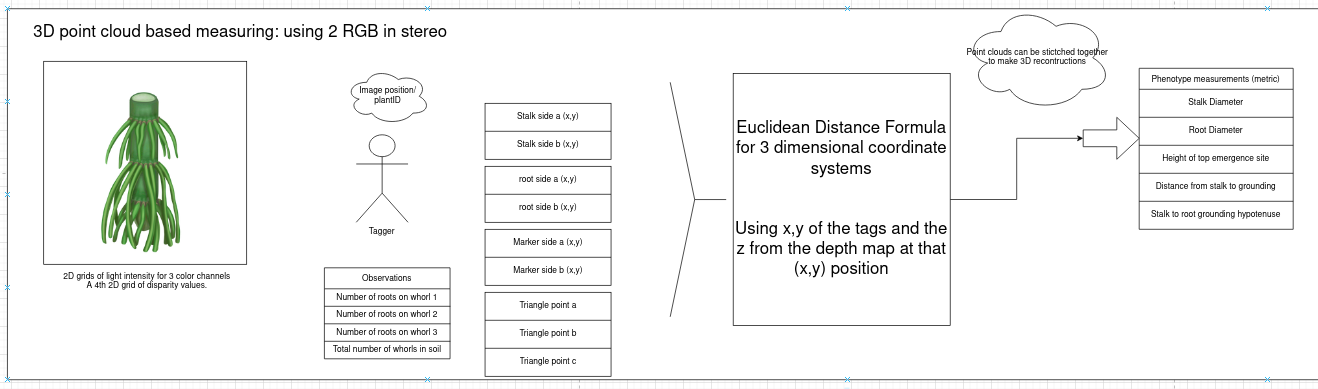
\includegraphics{the_matrix_files/image.png}

    Using this as a reference we can list the specific challenges that come
with collecting this data.

\begin{itemize}
\tightlist
\item
  Field traversal =\textgreater{} Who or what will be traversing where?
\item
  Modality of measurement =\textgreater{} Calipers, 2D distance, 3D
  distance? (The how)
\item
  Spatiotemporal data =\textgreater{} Where \& When is equally as
  important as the data being collected
\end{itemize}

Each of these will be a section, and each of those sections will lead to
entries in our table.

    Now we implement our scoring system. We'll grade everything on a 0-100
scale (0 = bad, 100 = good)\\
Here is a list of priorities: - Accuracy of measurements =\textgreater{}
Does this make the data higher or lower in quality? - Cost in man-hours
=\textgreater{} Does this make the testing day longer or shorter for the
researcher? - Cost of investment =\textgreater{} Is the cost of the
solution feasible? - Implementation time =\textgreater{} Is the time
investment required to build the solution feasible? - Time-to-data
=\textgreater{} Once testing day is done, will the data be available
sooner or later? - Potential value add =\textgreater{} Does this
solution have potential to add more insights to the research? -
Symbiosis =\textgreater{} Does using this solution work with the others
on the table?

    \begin{tcolorbox}[breakable, size=fbox, boxrule=1pt, pad at break*=1mm,colback=cellbackground, colframe=cellborder]
\prompt{In}{incolor}{1}{\boxspacing}
\begin{Verbatim}[commandchars=\\\{\}]
\PY{k+kn}{import} \PY{n+nn}{pandas} \PY{k}{as} \PY{n+nn}{pd}
\PY{k+kn}{from} \PY{n+nn}{IPython}\PY{n+nn}{.}\PY{n+nn}{display} \PY{k+kn}{import} \PY{n}{display}

\PY{c+c1}{\PYZsh{} Create an empty dataframe with the specified header}
\PY{n}{df} \PY{o}{=} \PY{n}{pd}\PY{o}{.}\PY{n}{DataFrame}\PY{p}{(}\PY{n}{columns}\PY{o}{=}\PY{p}{[}\PY{l+s+s1}{\PYZsq{}}\PY{l+s+s1}{Problem}\PY{l+s+s1}{\PYZsq{}}\PY{p}{,} \PY{l+s+s1}{\PYZsq{}}\PY{l+s+s1}{Solution}\PY{l+s+s1}{\PYZsq{}}\PY{p}{,} \PY{l+s+s1}{\PYZsq{}}\PY{l+s+s1}{Accuracy Score}\PY{l+s+s1}{\PYZsq{}}\PY{p}{,} \PY{l+s+s1}{\PYZsq{}}\PY{l+s+s1}{Man\PYZhy{}hour Score}\PY{l+s+s1}{\PYZsq{}}\PY{p}{,} \PY{l+s+s1}{\PYZsq{}}\PY{l+s+s1}{Investment Cost Score}\PY{l+s+s1}{\PYZsq{}}\PY{p}{,} \PY{l+s+s1}{\PYZsq{}}\PY{l+s+s1}{Implementation Time Score}\PY{l+s+s1}{\PYZsq{}}\PY{p}{,} \PY{l+s+s1}{\PYZsq{}}\PY{l+s+s1}{Time\PYZhy{}to\PYZhy{}data Complexity}\PY{l+s+s1}{\PYZsq{}}\PY{p}{,} \PY{l+s+s1}{\PYZsq{}}\PY{l+s+s1}{Potential Value Score}\PY{l+s+s1}{\PYZsq{}}\PY{p}{,} \PY{l+s+s1}{\PYZsq{}}\PY{l+s+s1}{Symbiosis Score}\PY{l+s+s1}{\PYZsq{}}\PY{p}{]}\PY{p}{)}

\PY{c+c1}{\PYZsh{} Add an example row to the dataframe}
\PY{n}{df}\PY{o}{.}\PY{n}{loc}\PY{p}{[}\PY{n+nb}{len}\PY{p}{(}\PY{n}{df}\PY{p}{)}\PY{p}{]} \PY{o}{=} \PY{p}{\PYZob{}}
    \PY{l+s+s1}{\PYZsq{}}\PY{l+s+s1}{Problem}\PY{l+s+s1}{\PYZsq{}}\PY{p}{:} \PY{l+s+s1}{\PYZsq{}}\PY{l+s+s1}{Sample Problem}\PY{l+s+s1}{\PYZsq{}}\PY{p}{,}
    \PY{l+s+s1}{\PYZsq{}}\PY{l+s+s1}{Solution}\PY{l+s+s1}{\PYZsq{}}\PY{p}{:} \PY{l+s+s1}{\PYZsq{}}\PY{l+s+s1}{Sample Solution}\PY{l+s+s1}{\PYZsq{}}\PY{p}{,}
    \PY{l+s+s1}{\PYZsq{}}\PY{l+s+s1}{Accuracy Score}\PY{l+s+s1}{\PYZsq{}}\PY{p}{:} \PY{l+m+mi}{0}\PY{p}{,}
    \PY{l+s+s1}{\PYZsq{}}\PY{l+s+s1}{Man\PYZhy{}hour Score}\PY{l+s+s1}{\PYZsq{}}\PY{p}{:} \PY{l+m+mi}{0}\PY{p}{,}
    \PY{l+s+s1}{\PYZsq{}}\PY{l+s+s1}{Investment Cost Score}\PY{l+s+s1}{\PYZsq{}}\PY{p}{:} \PY{l+m+mi}{0}\PY{p}{,}
    \PY{l+s+s1}{\PYZsq{}}\PY{l+s+s1}{Implementation Time Score}\PY{l+s+s1}{\PYZsq{}}\PY{p}{:} \PY{l+m+mi}{0}\PY{p}{,}
    \PY{l+s+s1}{\PYZsq{}}\PY{l+s+s1}{Time\PYZhy{}to\PYZhy{}data Complexity}\PY{l+s+s1}{\PYZsq{}}\PY{p}{:} \PY{l+m+mi}{0}\PY{p}{,}
    \PY{l+s+s1}{\PYZsq{}}\PY{l+s+s1}{Potential Value Score}\PY{l+s+s1}{\PYZsq{}}\PY{p}{:} \PY{l+m+mi}{0}\PY{p}{,}
    \PY{l+s+s1}{\PYZsq{}}\PY{l+s+s1}{Symbiosis Score}\PY{l+s+s1}{\PYZsq{}}\PY{p}{:} \PY{l+m+mi}{0}
\PY{p}{\PYZcb{}}

\PY{c+c1}{\PYZsh{} Print the dataframe using the display function}
\PY{n}{display}\PY{p}{(}\PY{n}{df}\PY{p}{)}
\end{Verbatim}
\end{tcolorbox}

    
    \begin{Verbatim}[commandchars=\\\{\}]
          Problem         Solution  Accuracy Score  Man-hour Score  \textbackslash{}
0  Sample Problem  Sample Solution               0               0   

   Investment Cost Score  Implementation Time Score  Time-to-data Complexity  \textbackslash{}
0                      0                          0                        0   

   Potential Value Score  Symbiosis Score  
0                      0                0  
    \end{Verbatim}

    
    \hypertarget{section-2-problems-solutions}{%
\subsubsection{Section 2: Problems \&
Solutions}\label{section-2-problems-solutions}}

\hypertarget{section-2.1-field-traversal}{%
\paragraph{Section 2.1: Field
Traversal}\label{section-2.1-field-traversal}}

The ``who or what'' of the data collection problem.

The first entry to consider is for fully manual data collection. An
extremely dedicated researcher with calipers and notebook in hand
decides to gather brace root phenotypes (all 9 measurements and
observations, 2 more will be calculated after the fact).

    \begin{tcolorbox}[breakable, size=fbox, boxrule=1pt, pad at break*=1mm,colback=cellbackground, colframe=cellborder]
\prompt{In}{incolor}{2}{\boxspacing}
\begin{Verbatim}[commandchars=\\\{\}]
\PY{n}{df}\PY{o}{.}\PY{n}{loc}\PY{p}{[}\PY{n+nb}{len}\PY{p}{(}\PY{n}{df}\PY{p}{)}\PY{p}{]} \PY{o}{=} \PY{p}{\PYZob{}}
    \PY{l+s+s1}{\PYZsq{}}\PY{l+s+s1}{Problem}\PY{l+s+s1}{\PYZsq{}}\PY{p}{:} \PY{l+s+s1}{\PYZsq{}}\PY{l+s+s1}{2.1 Field Traversal}\PY{l+s+s1}{\PYZsq{}}\PY{p}{,}
    \PY{l+s+s1}{\PYZsq{}}\PY{l+s+s1}{Solution}\PY{l+s+s1}{\PYZsq{}}\PY{p}{:} \PY{l+s+s1}{\PYZsq{}}\PY{l+s+s1}{Fully Manual}\PY{l+s+s1}{\PYZsq{}}\PY{p}{,}
    \PY{l+s+s1}{\PYZsq{}}\PY{l+s+s1}{Accuracy Score}\PY{l+s+s1}{\PYZsq{}}\PY{p}{:} \PY{l+m+mi}{50}\PY{p}{,} \PY{c+c1}{\PYZsh{}humans aren\PYZsq{}t accurate, yet somehow we still trust them }
    \PY{l+s+s1}{\PYZsq{}}\PY{l+s+s1}{Man\PYZhy{}hour Score}\PY{l+s+s1}{\PYZsq{}}\PY{p}{:} \PY{l+m+mi}{0}\PY{p}{,}  \PY{c+c1}{\PYZsh{}humans aren\PYZsq{}t cheap, at 5 minutes per plant, the data that can be collected on one day is limited}
    \PY{l+s+s1}{\PYZsq{}}\PY{l+s+s1}{Investment Cost Score}\PY{l+s+s1}{\PYZsq{}}\PY{p}{:} \PY{l+m+mi}{80}\PY{p}{,} \PY{c+c1}{\PYZsh{}The man hours are the most expensive part of this process, but plot \PYZam{} plant markers would be required as well}
    \PY{l+s+s1}{\PYZsq{}}\PY{l+s+s1}{Implementation Time Score}\PY{l+s+s1}{\PYZsq{}}\PY{p}{:} \PY{l+m+mi}{90}\PY{p}{,} \PY{c+c1}{\PYZsh{}Theres nothing to implement, but making sure things are consistent would require documentation }
    \PY{l+s+s1}{\PYZsq{}}\PY{l+s+s1}{Time\PYZhy{}to\PYZhy{}data Complexity}\PY{l+s+s1}{\PYZsq{}}\PY{p}{:} \PY{l+m+mi}{80}\PY{p}{,} \PY{c+c1}{\PYZsh{}If you ignore the time to digitize, time to data is low}
    \PY{l+s+s1}{\PYZsq{}}\PY{l+s+s1}{Potential Value Score}\PY{l+s+s1}{\PYZsq{}}\PY{p}{:} \PY{l+m+mi}{0}\PY{p}{,} \PY{c+c1}{\PYZsh{}There is no extra data to tap into}
    \PY{l+s+s1}{\PYZsq{}}\PY{l+s+s1}{Symbiosis Score}\PY{l+s+s1}{\PYZsq{}}\PY{p}{:} \PY{l+m+mi}{100}  \PY{c+c1}{\PYZsh{}Highly symbiotic, we\PYZsq{}ve had to do this when validating other solutions before.  }
\PY{p}{\PYZcb{}}
\end{Verbatim}
\end{tcolorbox}

    Now lets consider the case in which we develop a tool that allows the
researcher to gather this data one plant at a time, 10 seconds per
plant, and the method requires post processing to actually extract the
phenotype data after the fact.

    \begin{tcolorbox}[breakable, size=fbox, boxrule=1pt, pad at break*=1mm,colback=cellbackground, colframe=cellborder]
\prompt{In}{incolor}{3}{\boxspacing}
\begin{Verbatim}[commandchars=\\\{\}]
\PY{n}{df}\PY{o}{.}\PY{n}{loc}\PY{p}{[}\PY{n+nb}{len}\PY{p}{(}\PY{n}{df}\PY{p}{)}\PY{p}{]} \PY{o}{=} \PY{p}{\PYZob{}}
    \PY{l+s+s1}{\PYZsq{}}\PY{l+s+s1}{Problem}\PY{l+s+s1}{\PYZsq{}}\PY{p}{:} \PY{l+s+s1}{\PYZsq{}}\PY{l+s+s1}{2.1 Field Traversal}\PY{l+s+s1}{\PYZsq{}}\PY{p}{,}
    \PY{l+s+s1}{\PYZsq{}}\PY{l+s+s1}{Solution}\PY{l+s+s1}{\PYZsq{}}\PY{p}{:} \PY{l+s+s1}{\PYZsq{}}\PY{l+s+s1}{Manual \PYZhy{} tool assisted \PYZhy{} post processed}\PY{l+s+s1}{\PYZsq{}}\PY{p}{,}
    \PY{l+s+s1}{\PYZsq{}}\PY{l+s+s1}{Accuracy Score}\PY{l+s+s1}{\PYZsq{}}\PY{p}{:} \PY{l+m+mi}{90}\PY{p}{,} \PY{c+c1}{\PYZsh{}Offloading the measurement to something more consistent }
    \PY{l+s+s1}{\PYZsq{}}\PY{l+s+s1}{Man\PYZhy{}hour Score}\PY{l+s+s1}{\PYZsq{}}\PY{p}{:} \PY{l+m+mi}{60}\PY{p}{,}  \PY{c+c1}{\PYZsh{}The man hours in the field are optimized, but there remains a hidden cost to post processing }
    \PY{l+s+s1}{\PYZsq{}}\PY{l+s+s1}{Investment Cost Score}\PY{l+s+s1}{\PYZsq{}}\PY{p}{:} \PY{l+m+mi}{40}\PY{p}{,} \PY{c+c1}{\PYZsh{}Tools have cost, post processing pipelines have cost}
    \PY{l+s+s1}{\PYZsq{}}\PY{l+s+s1}{Implementation Time Score}\PY{l+s+s1}{\PYZsq{}}\PY{p}{:} \PY{l+m+mi}{60}\PY{p}{,} \PY{c+c1}{\PYZsh{}handheld tools are easy to implement, but they and the pipelines would still need to be maintained  }
    \PY{l+s+s1}{\PYZsq{}}\PY{l+s+s1}{Time\PYZhy{}to\PYZhy{}data Complexity}\PY{l+s+s1}{\PYZsq{}}\PY{p}{:} \PY{l+m+mi}{20}\PY{p}{,} \PY{c+c1}{\PYZsh{}procrastination is a devil and data will sit unprocessed}
    \PY{l+s+s1}{\PYZsq{}}\PY{l+s+s1}{Potential Value Score}\PY{l+s+s1}{\PYZsq{}}\PY{p}{:} \PY{l+m+mi}{50}\PY{p}{,} \PY{c+c1}{\PYZsh{}the more potential built in the higher the cost of post processing}
    \PY{l+s+s1}{\PYZsq{}}\PY{l+s+s1}{Symbiosis Score}\PY{l+s+s1}{\PYZsq{}}\PY{p}{:} \PY{l+m+mi}{20}  \PY{c+c1}{\PYZsh{}This method would pidgeon hole us with the constraint of having to be a maneuverable tool for the field  }
\PY{p}{\PYZcb{}}
\end{Verbatim}
\end{tcolorbox}

    Now lets move away from humans, and towards robotics. The simple goal of
robotics is to remove the human. But the drawbacks come in a dramatic
lack of being able to adapt on the fly, and massive amounts of
investment in time and money.

    \begin{tcolorbox}[breakable, size=fbox, boxrule=1pt, pad at break*=1mm,colback=cellbackground, colframe=cellborder]
\prompt{In}{incolor}{4}{\boxspacing}
\begin{Verbatim}[commandchars=\\\{\}]
\PY{n}{df}\PY{o}{.}\PY{n}{loc}\PY{p}{[}\PY{n+nb}{len}\PY{p}{(}\PY{n}{df}\PY{p}{)}\PY{p}{]} \PY{o}{=} \PY{p}{\PYZob{}}
    \PY{l+s+s1}{\PYZsq{}}\PY{l+s+s1}{Problem}\PY{l+s+s1}{\PYZsq{}}\PY{p}{:} \PY{l+s+s1}{\PYZsq{}}\PY{l+s+s1}{2.1 Field Traversal}\PY{l+s+s1}{\PYZsq{}}\PY{p}{,}
    \PY{l+s+s1}{\PYZsq{}}\PY{l+s+s1}{Solution}\PY{l+s+s1}{\PYZsq{}}\PY{p}{:} \PY{l+s+s1}{\PYZsq{}}\PY{l+s+s1}{Robotic \PYZhy{} ground\PYZhy{}based}\PY{l+s+s1}{\PYZsq{}}\PY{p}{,}
    \PY{l+s+s1}{\PYZsq{}}\PY{l+s+s1}{Accuracy Score}\PY{l+s+s1}{\PYZsq{}}\PY{p}{:} \PY{l+m+mi}{90}\PY{p}{,} \PY{c+c1}{\PYZsh{}Offloading the measurement to something more consistent }
    \PY{l+s+s1}{\PYZsq{}}\PY{l+s+s1}{Man\PYZhy{}hour Score}\PY{l+s+s1}{\PYZsq{}}\PY{p}{:} \PY{l+m+mi}{90}\PY{p}{,}  \PY{c+c1}{\PYZsh{}Ideally, the need for human effort would be greatly reduced, but maintanance would be required}
    \PY{l+s+s1}{\PYZsq{}}\PY{l+s+s1}{Investment Cost Score}\PY{l+s+s1}{\PYZsq{}}\PY{p}{:} \PY{l+m+mi}{20}\PY{p}{,} \PY{c+c1}{\PYZsh{}Robots are expensive up front, with the reward of reduced labor costs over time}
    \PY{l+s+s1}{\PYZsq{}}\PY{l+s+s1}{Implementation Time Score}\PY{l+s+s1}{\PYZsq{}}\PY{p}{:} \PY{l+m+mi}{5}\PY{p}{,} \PY{c+c1}{\PYZsh{}maintaining hardware, maintaining software, and maintaining the data pipeline, all require time }
    \PY{l+s+s1}{\PYZsq{}}\PY{l+s+s1}{Time\PYZhy{}to\PYZhy{}data Complexity}\PY{l+s+s1}{\PYZsq{}}\PY{p}{:} \PY{l+m+mi}{90}\PY{p}{,} \PY{c+c1}{\PYZsh{}Ideally, a pipeline can be in place to make the data available immediately}
    \PY{l+s+s1}{\PYZsq{}}\PY{l+s+s1}{Potential Value Score}\PY{l+s+s1}{\PYZsq{}}\PY{p}{:} \PY{l+m+mi}{80}\PY{p}{,} \PY{c+c1}{\PYZsh{}Depending on the data collected, the potential value could be higher than more selective methods}
    \PY{l+s+s1}{\PYZsq{}}\PY{l+s+s1}{Symbiosis Score}\PY{l+s+s1}{\PYZsq{}}\PY{p}{:} \PY{l+m+mi}{0}  \PY{c+c1}{\PYZsh{} with so much investment upfront, its a hard ask to entertain other solutions at the same time  }
\PY{p}{\PYZcb{}}
\end{Verbatim}
\end{tcolorbox}

    Drone robotics projects in agriculture also exist, but they rarely
geared towards phenotyping, usually pest control. Operating a drone
subcanopy would be damn near impossible.

    \begin{tcolorbox}[breakable, size=fbox, boxrule=1pt, pad at break*=1mm,colback=cellbackground, colframe=cellborder]
\prompt{In}{incolor}{5}{\boxspacing}
\begin{Verbatim}[commandchars=\\\{\}]
\PY{n}{df}\PY{o}{.}\PY{n}{loc}\PY{p}{[}\PY{n+nb}{len}\PY{p}{(}\PY{n}{df}\PY{p}{)}\PY{p}{]} \PY{o}{=} \PY{p}{\PYZob{}}
    \PY{l+s+s1}{\PYZsq{}}\PY{l+s+s1}{Problem}\PY{l+s+s1}{\PYZsq{}}\PY{p}{:} \PY{l+s+s1}{\PYZsq{}}\PY{l+s+s1}{2.1 Field Traversal}\PY{l+s+s1}{\PYZsq{}}\PY{p}{,}
    \PY{l+s+s1}{\PYZsq{}}\PY{l+s+s1}{Solution}\PY{l+s+s1}{\PYZsq{}}\PY{p}{:} \PY{l+s+s1}{\PYZsq{}}\PY{l+s+s1}{Robotic \PYZhy{} drone}\PY{l+s+s1}{\PYZsq{}}\PY{p}{,}
    \PY{l+s+s1}{\PYZsq{}}\PY{l+s+s1}{Accuracy Score}\PY{l+s+s1}{\PYZsq{}}\PY{p}{:} \PY{l+m+mi}{5}\PY{p}{,} \PY{c+c1}{\PYZsh{}The ability of the sensors would be greatly limited by the payload capacity of the drone }
    \PY{l+s+s1}{\PYZsq{}}\PY{l+s+s1}{Man\PYZhy{}hour Score}\PY{l+s+s1}{\PYZsq{}}\PY{p}{:} \PY{l+m+mi}{90}\PY{p}{,}  \PY{c+c1}{\PYZsh{}Ideally, the need for human effort would be greatly reduced, but maintanance would be required}
    \PY{l+s+s1}{\PYZsq{}}\PY{l+s+s1}{Investment Cost Score}\PY{l+s+s1}{\PYZsq{}}\PY{p}{:} \PY{l+m+mi}{20}\PY{p}{,} \PY{c+c1}{\PYZsh{}Robots are expensive up front, with the reward of reduced labor costs over time}
    \PY{l+s+s1}{\PYZsq{}}\PY{l+s+s1}{Implementation Time Score}\PY{l+s+s1}{\PYZsq{}}\PY{p}{:} \PY{l+m+mi}{1}\PY{p}{,} \PY{c+c1}{\PYZsh{}The shear engineering work that would have to go into this would be staggering }
    \PY{l+s+s1}{\PYZsq{}}\PY{l+s+s1}{Time\PYZhy{}to\PYZhy{}data Complexity}\PY{l+s+s1}{\PYZsq{}}\PY{p}{:} \PY{l+m+mi}{80}\PY{p}{,} \PY{c+c1}{\PYZsh{}Processing could never happen on\PYZhy{}board, there would need to be a pipeline for after}
    \PY{l+s+s1}{\PYZsq{}}\PY{l+s+s1}{Potential Value Score}\PY{l+s+s1}{\PYZsq{}}\PY{p}{:} \PY{l+m+mi}{80}\PY{p}{,} \PY{c+c1}{\PYZsh{}Depending on the data collected, the potential value could be higher than more selective methods}
    \PY{l+s+s1}{\PYZsq{}}\PY{l+s+s1}{Symbiosis Score}\PY{l+s+s1}{\PYZsq{}}\PY{p}{:} \PY{l+m+mi}{0}  \PY{c+c1}{\PYZsh{} This is just a bad idea  }
\PY{p}{\PYZcb{}}
\end{Verbatim}
\end{tcolorbox}

    \hypertarget{section-2.2-modality-of-measurement}{%
\paragraph{Section 2.2: Modality of
Measurement}\label{section-2.2-modality-of-measurement}}

Now we can start to discuss the most complex part of the problem.\\
Like the previous section, we'll start with the most manual method.
Calipers.\\
Using a set of calipers and a ruler, a researcher must measure: - Stalk
diameter - Brace root diameter (one per plant) - Height of the top whorl
with roots in the soil - Distance from stalk to root grounding point
(left) - Distance from stalk to root grounding point (right) - Number of
roots per whorl - Number of whorls in the soil - Plant Identifier
(location in the field)

    \begin{tcolorbox}[breakable, size=fbox, boxrule=1pt, pad at break*=1mm,colback=cellbackground, colframe=cellborder]
\prompt{In}{incolor}{6}{\boxspacing}
\begin{Verbatim}[commandchars=\\\{\}]
\PY{n}{df}\PY{o}{.}\PY{n}{loc}\PY{p}{[}\PY{n+nb}{len}\PY{p}{(}\PY{n}{df}\PY{p}{)}\PY{p}{]} \PY{o}{=} \PY{p}{\PYZob{}}
    \PY{l+s+s1}{\PYZsq{}}\PY{l+s+s1}{Problem}\PY{l+s+s1}{\PYZsq{}}\PY{p}{:} \PY{l+s+s1}{\PYZsq{}}\PY{l+s+s1}{2.2 Modality of Measurement}\PY{l+s+s1}{\PYZsq{}}\PY{p}{,}
    \PY{l+s+s1}{\PYZsq{}}\PY{l+s+s1}{Solution}\PY{l+s+s1}{\PYZsq{}}\PY{p}{:} \PY{l+s+s1}{\PYZsq{}}\PY{l+s+s1}{Fully Manual}\PY{l+s+s1}{\PYZsq{}}\PY{p}{,}
    \PY{l+s+s1}{\PYZsq{}}\PY{l+s+s1}{Accuracy Score}\PY{l+s+s1}{\PYZsq{}}\PY{p}{:} \PY{l+m+mi}{50}\PY{p}{,} \PY{c+c1}{\PYZsh{}humans aren\PYZsq{}t accurate, yet somehow we still trust them }
    \PY{l+s+s1}{\PYZsq{}}\PY{l+s+s1}{Man\PYZhy{}hour Score}\PY{l+s+s1}{\PYZsq{}}\PY{p}{:} \PY{l+m+mi}{5}\PY{p}{,}  \PY{c+c1}{\PYZsh{}This is a very slow process}
    \PY{l+s+s1}{\PYZsq{}}\PY{l+s+s1}{Investment Cost Score}\PY{l+s+s1}{\PYZsq{}}\PY{p}{:} \PY{l+m+mi}{80}\PY{p}{,} \PY{c+c1}{\PYZsh{}The man hours are the most expensive part of this process, but plot \PYZam{} plant markers would be required as well}
    \PY{l+s+s1}{\PYZsq{}}\PY{l+s+s1}{Implementation Time Score}\PY{l+s+s1}{\PYZsq{}}\PY{p}{:} \PY{l+m+mi}{90}\PY{p}{,} \PY{c+c1}{\PYZsh{}theres nothing to implement, but making sure things are consistent would require documentation }
    \PY{l+s+s1}{\PYZsq{}}\PY{l+s+s1}{Time\PYZhy{}to\PYZhy{}data Complexity}\PY{l+s+s1}{\PYZsq{}}\PY{p}{:} \PY{l+m+mi}{5}\PY{p}{,} \PY{c+c1}{\PYZsh{}once digitized, the data would be available}
    \PY{l+s+s1}{\PYZsq{}}\PY{l+s+s1}{Potential Value Score}\PY{l+s+s1}{\PYZsq{}}\PY{p}{:} \PY{l+m+mi}{5}\PY{p}{,} \PY{c+c1}{\PYZsh{}There is no extra data to tap into}
    \PY{l+s+s1}{\PYZsq{}}\PY{l+s+s1}{Symbiosis Score}\PY{l+s+s1}{\PYZsq{}}\PY{p}{:} \PY{l+m+mi}{100}  \PY{c+c1}{\PYZsh{}Highly symbiotic, we\PYZsq{}ve had to do this when validating other solutions before.   }
\PY{p}{\PYZcb{}}
\end{Verbatim}
\end{tcolorbox}

    Another method of measurement is using 2 dimensional images. To get a
measurement from an image a few choices have to be made.\\
Option 1: each image has a reference marker with a known size, from
this, we can get pixels per metric ratio and use the pythagorean
distance formula for 2D coordinate systems to get our measurements.
Heres a diagram of that workflow:
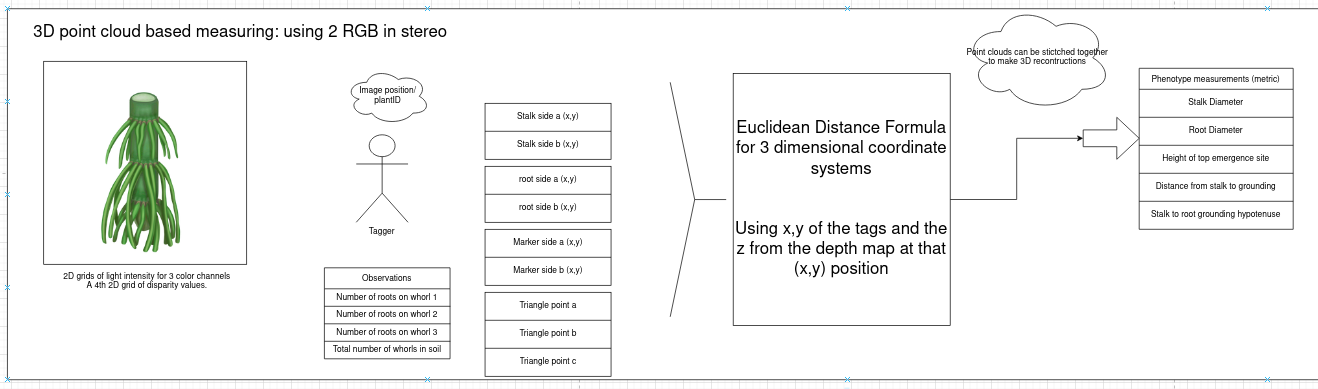
\includegraphics{the_matrix_files/image.png}

    \begin{tcolorbox}[breakable, size=fbox, boxrule=1pt, pad at break*=1mm,colback=cellbackground, colframe=cellborder]
\prompt{In}{incolor}{7}{\boxspacing}
\begin{Verbatim}[commandchars=\\\{\}]
\PY{n}{df}\PY{o}{.}\PY{n}{loc}\PY{p}{[}\PY{n+nb}{len}\PY{p}{(}\PY{n}{df}\PY{p}{)}\PY{p}{]} \PY{o}{=} \PY{p}{\PYZob{}}
    \PY{l+s+s1}{\PYZsq{}}\PY{l+s+s1}{Problem}\PY{l+s+s1}{\PYZsq{}}\PY{p}{:} \PY{l+s+s1}{\PYZsq{}}\PY{l+s+s1}{2.2 Modality of Measurement}\PY{l+s+s1}{\PYZsq{}}\PY{p}{,}
    \PY{l+s+s1}{\PYZsq{}}\PY{l+s+s1}{Solution}\PY{l+s+s1}{\PYZsq{}}\PY{p}{:} \PY{l+s+s1}{\PYZsq{}}\PY{l+s+s1}{2D Images \PYZhy{} Scale markers}\PY{l+s+s1}{\PYZsq{}}\PY{p}{,}
    \PY{l+s+s1}{\PYZsq{}}\PY{l+s+s1}{Accuracy Score}\PY{l+s+s1}{\PYZsq{}}\PY{p}{:} \PY{l+m+mi}{90}\PY{p}{,} \PY{c+c1}{\PYZsh{}Once validated, this method is consistent and accurate }
    \PY{l+s+s1}{\PYZsq{}}\PY{l+s+s1}{Man\PYZhy{}hour Score}\PY{l+s+s1}{\PYZsq{}}\PY{p}{:} \PY{l+m+mi}{40}\PY{p}{,}  \PY{c+c1}{\PYZsh{}someone has to take the pictures, and most importantly someone has to put the scale markers out}
    \PY{l+s+s1}{\PYZsq{}}\PY{l+s+s1}{Investment Cost Score}\PY{l+s+s1}{\PYZsq{}}\PY{p}{:} \PY{l+m+mi}{80}\PY{p}{,} \PY{c+c1}{\PYZsh{}The man hours are the most expensive part of this process, but plot \PYZam{} plant markers would be required as well}
    \PY{l+s+s1}{\PYZsq{}}\PY{l+s+s1}{Implementation Time Score}\PY{l+s+s1}{\PYZsq{}}\PY{p}{:} \PY{l+m+mi}{70}\PY{p}{,} \PY{c+c1}{\PYZsh{}The pipeline to convert these images to our desired data could be implemented and optimizes quickly }
    \PY{l+s+s1}{\PYZsq{}}\PY{l+s+s1}{Time\PYZhy{}to\PYZhy{}data Complexity}\PY{l+s+s1}{\PYZsq{}}\PY{p}{:} \PY{l+m+mi}{20}\PY{p}{,} \PY{c+c1}{\PYZsh{}Digitization is automatic, but the post processing pipline would be heavier}
    \PY{l+s+s1}{\PYZsq{}}\PY{l+s+s1}{Potential Value Score}\PY{l+s+s1}{\PYZsq{}}\PY{p}{:} \PY{l+m+mi}{50}\PY{p}{,} \PY{c+c1}{\PYZsh{}If new requirements from this data arise after the fact, there is potential to re\PYZhy{}analyse old data}
    \PY{l+s+s1}{\PYZsq{}}\PY{l+s+s1}{Symbiosis Score}\PY{l+s+s1}{\PYZsq{}}\PY{p}{:} \PY{l+m+mi}{60}  \PY{c+c1}{\PYZsh{}This solution can be used in conjunction with other solutions with some crafty implementation   }
\PY{p}{\PYZcb{}}
\end{Verbatim}
\end{tcolorbox}

    By fixing a few things such as: - Focal length of the camera lens -
Distance from the lens to the subject - Aperture setting of the camera
lens

We can calculate one pixel per metric ratio and carry that throughout
the field.

    \begin{tcolorbox}[breakable, size=fbox, boxrule=1pt, pad at break*=1mm,colback=cellbackground, colframe=cellborder]
\prompt{In}{incolor}{8}{\boxspacing}
\begin{Verbatim}[commandchars=\\\{\}]
\PY{n}{df}\PY{o}{.}\PY{n}{loc}\PY{p}{[}\PY{n+nb}{len}\PY{p}{(}\PY{n}{df}\PY{p}{)}\PY{p}{]} \PY{o}{=} \PY{p}{\PYZob{}}
    \PY{l+s+s1}{\PYZsq{}}\PY{l+s+s1}{Problem}\PY{l+s+s1}{\PYZsq{}}\PY{p}{:} \PY{l+s+s1}{\PYZsq{}}\PY{l+s+s1}{2.2 Modality of Measurement}\PY{l+s+s1}{\PYZsq{}}\PY{p}{,}
    \PY{l+s+s1}{\PYZsq{}}\PY{l+s+s1}{Solution}\PY{l+s+s1}{\PYZsq{}}\PY{p}{:} \PY{l+s+s1}{\PYZsq{}}\PY{l+s+s1}{2D Images \PYZhy{} fixed}\PY{l+s+s1}{\PYZsq{}}\PY{p}{,}
    \PY{l+s+s1}{\PYZsq{}}\PY{l+s+s1}{Accuracy Score}\PY{l+s+s1}{\PYZsq{}}\PY{p}{:} \PY{l+m+mi}{90}\PY{p}{,} \PY{c+c1}{\PYZsh{}Once validated, this method is consistent and accurate }
    \PY{l+s+s1}{\PYZsq{}}\PY{l+s+s1}{Man\PYZhy{}hour Score}\PY{l+s+s1}{\PYZsq{}}\PY{p}{:} \PY{l+m+mi}{40}\PY{p}{,}  \PY{c+c1}{\PYZsh{}someone has to take the pictures}
    \PY{l+s+s1}{\PYZsq{}}\PY{l+s+s1}{Investment Cost Score}\PY{l+s+s1}{\PYZsq{}}\PY{p}{:} \PY{l+m+mi}{80}\PY{p}{,} \PY{c+c1}{\PYZsh{} once you have a camera and a consistent distance, the rest is easy}
    \PY{l+s+s1}{\PYZsq{}}\PY{l+s+s1}{Implementation Time Score}\PY{l+s+s1}{\PYZsq{}}\PY{p}{:} \PY{l+m+mi}{70}\PY{p}{,} \PY{c+c1}{\PYZsh{}The pipeline to convert these images to our desired data could be implemented and optimized quickly }
    \PY{l+s+s1}{\PYZsq{}}\PY{l+s+s1}{Time\PYZhy{}to\PYZhy{}data Complexity}\PY{l+s+s1}{\PYZsq{}}\PY{p}{:} \PY{l+m+mi}{40}\PY{p}{,} \PY{c+c1}{\PYZsh{}Digitization is automatic, removing the scale markers would simplify the analysis}
    \PY{l+s+s1}{\PYZsq{}}\PY{l+s+s1}{Potential Value Score}\PY{l+s+s1}{\PYZsq{}}\PY{p}{:} \PY{l+m+mi}{50}\PY{p}{,} \PY{c+c1}{\PYZsh{}If new requirements from this data arise after the fact, there is potential to re\PYZhy{}analyse old data}
    \PY{l+s+s1}{\PYZsq{}}\PY{l+s+s1}{Symbiosis Score}\PY{l+s+s1}{\PYZsq{}}\PY{p}{:} \PY{l+m+mi}{60}  \PY{c+c1}{\PYZsh{}This solution can be used in conjunction with other solutions with some crafty implementation   }
\PY{p}{\PYZcb{}}
\end{Verbatim}
\end{tcolorbox}

    Now what if me added a 3rd dimension? With cameras, we can achieve this
by adding a second image taken at the same time and using the distance
between the sensors as our way to calculate scale. This would create a
point cloud image of 4 layers, 3 for color and a 4th for depth from the
sensor. Here is a diagram of that workflow:
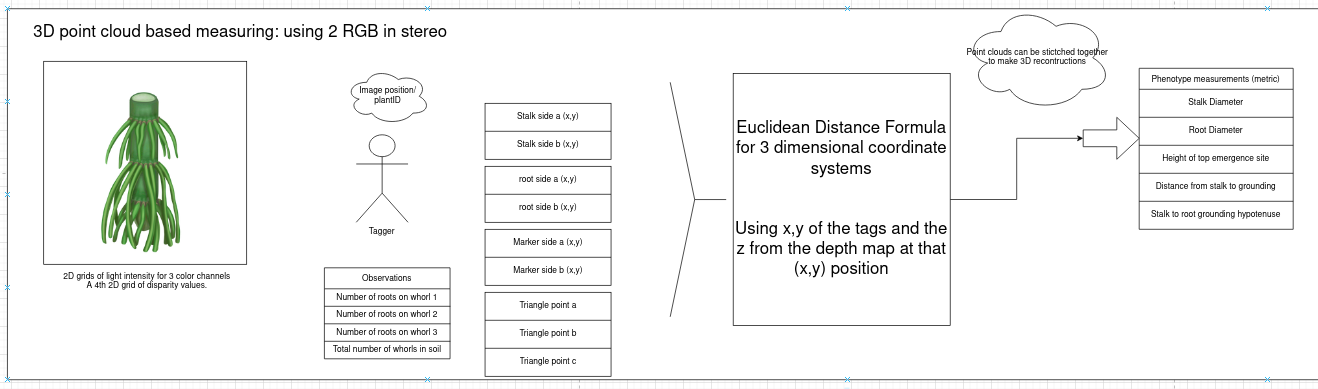
\includegraphics{the_matrix_files/image.png}

    \begin{tcolorbox}[breakable, size=fbox, boxrule=1pt, pad at break*=1mm,colback=cellbackground, colframe=cellborder]
\prompt{In}{incolor}{9}{\boxspacing}
\begin{Verbatim}[commandchars=\\\{\}]
\PY{n}{df}\PY{o}{.}\PY{n}{loc}\PY{p}{[}\PY{n+nb}{len}\PY{p}{(}\PY{n}{df}\PY{p}{)}\PY{p}{]} \PY{o}{=} \PY{p}{\PYZob{}}
    \PY{l+s+s1}{\PYZsq{}}\PY{l+s+s1}{Problem}\PY{l+s+s1}{\PYZsq{}}\PY{p}{:} \PY{l+s+s1}{\PYZsq{}}\PY{l+s+s1}{2.2 Modality of Measurement}\PY{l+s+s1}{\PYZsq{}}\PY{p}{,}
    \PY{l+s+s1}{\PYZsq{}}\PY{l+s+s1}{Solution}\PY{l+s+s1}{\PYZsq{}}\PY{p}{:} \PY{l+s+s1}{\PYZsq{}}\PY{l+s+s1}{3D Images \PYZhy{} RGB\PYZhy{}D}\PY{l+s+s1}{\PYZsq{}}\PY{p}{,}
    \PY{l+s+s1}{\PYZsq{}}\PY{l+s+s1}{Accuracy Score}\PY{l+s+s1}{\PYZsq{}}\PY{p}{:} \PY{l+m+mi}{80}\PY{p}{,} \PY{c+c1}{\PYZsh{}Once validated, this method is consistent and accurate, but more suseptible to noise }
    \PY{l+s+s1}{\PYZsq{}}\PY{l+s+s1}{Man\PYZhy{}hour Score}\PY{l+s+s1}{\PYZsq{}}\PY{p}{:} \PY{l+m+mi}{40}\PY{p}{,}  \PY{c+c1}{\PYZsh{}someone has to take the pictures}
    \PY{l+s+s1}{\PYZsq{}}\PY{l+s+s1}{Investment Cost Score}\PY{l+s+s1}{\PYZsq{}}\PY{p}{:} \PY{l+m+mi}{70}\PY{p}{,} \PY{c+c1}{\PYZsh{} double the cameras double the cost, scale markers no longer required}
    \PY{l+s+s1}{\PYZsq{}}\PY{l+s+s1}{Implementation Time Score}\PY{l+s+s1}{\PYZsq{}}\PY{p}{:} \PY{l+m+mi}{60}\PY{p}{,} \PY{c+c1}{\PYZsh{}more configuration required to the cameras}
    \PY{l+s+s1}{\PYZsq{}}\PY{l+s+s1}{Time\PYZhy{}to\PYZhy{}data Complexity}\PY{l+s+s1}{\PYZsq{}}\PY{p}{:} \PY{l+m+mi}{60}\PY{p}{,} \PY{c+c1}{\PYZsh{}Adding a third dimension allows for more optimiztion of the processing pipeline}
    \PY{l+s+s1}{\PYZsq{}}\PY{l+s+s1}{Potential Value Score}\PY{l+s+s1}{\PYZsq{}}\PY{p}{:} \PY{l+m+mi}{70}\PY{p}{,} \PY{c+c1}{\PYZsh{}We have the same potential for re\PYZhy{}analysis}
    \PY{l+s+s1}{\PYZsq{}}\PY{l+s+s1}{Symbiosis Score}\PY{l+s+s1}{\PYZsq{}}\PY{p}{:} \PY{l+m+mi}{60}  \PY{c+c1}{\PYZsh{}This solution can be used in conjunction with other solutions with some crafty implementation   }
\PY{p}{\PYZcb{}}
\end{Verbatim}
\end{tcolorbox}

    I should explain why the potential for pipeline optimization and
potential value is higher here.\\
In order to optimize this pipeline for minimizing Time-to-data, we will
have to train machine learning models on this data to solve a few
problems, the most important of which include: - Identifying individual
brace roots - Identifying stalks

If we can do that then we can calculate everything else from the output
of those 2 models.

By adding that third dimension the number of training parameters and
identifiable features greatly increases (in fact, it increases
exponentially). According to
\href{https://arxiv.org/pdf/2101.07612}{this paper} the efficiency of
the models also greatly increases.

So using 3D data could allow us to more easily discern each individual
brace root in the whorl, which can help us automate counting brace roots
and measuring them.

    Not all 3D data is RGB-D. There are other options. One of which is Light
Detection and Ranging (LiDAR). According to
\href{https://www.mdpi.com/2075-1702/11/1/48}{this paper} LiDAR is the
3rd most used sensor in agrcultural robotics. The working theory is that
a grid of laser can be projected out towards the subject and the
reflection of that grid back into the sensor will be a depth map.

However, its my opinion that there is an incompleteness to this data, as
there isn't a human viewable image in this data. LiDAR is often used in
conjunction with RGB

    \begin{tcolorbox}[breakable, size=fbox, boxrule=1pt, pad at break*=1mm,colback=cellbackground, colframe=cellborder]
\prompt{In}{incolor}{10}{\boxspacing}
\begin{Verbatim}[commandchars=\\\{\}]
\PY{n}{df}\PY{o}{.}\PY{n}{loc}\PY{p}{[}\PY{n+nb}{len}\PY{p}{(}\PY{n}{df}\PY{p}{)}\PY{p}{]} \PY{o}{=} \PY{p}{\PYZob{}}
    \PY{l+s+s1}{\PYZsq{}}\PY{l+s+s1}{Problem}\PY{l+s+s1}{\PYZsq{}}\PY{p}{:} \PY{l+s+s1}{\PYZsq{}}\PY{l+s+s1}{2.2 Modality of Measurement}\PY{l+s+s1}{\PYZsq{}}\PY{p}{,}
    \PY{l+s+s1}{\PYZsq{}}\PY{l+s+s1}{Solution}\PY{l+s+s1}{\PYZsq{}}\PY{p}{:} \PY{l+s+s1}{\PYZsq{}}\PY{l+s+s1}{Point Cloud \PYZhy{} LiDAR}\PY{l+s+s1}{\PYZsq{}}\PY{p}{,}
    \PY{l+s+s1}{\PYZsq{}}\PY{l+s+s1}{Accuracy Score}\PY{l+s+s1}{\PYZsq{}}\PY{p}{:} \PY{l+m+mi}{70}\PY{p}{,} \PY{c+c1}{\PYZsh{} possible noise problems}
    \PY{l+s+s1}{\PYZsq{}}\PY{l+s+s1}{Man\PYZhy{}hour Score}\PY{l+s+s1}{\PYZsq{}}\PY{p}{:} \PY{l+m+mi}{40}\PY{p}{,} \PY{c+c1}{\PYZsh{}same time requirement as other imaging teqniques}
    \PY{l+s+s1}{\PYZsq{}}\PY{l+s+s1}{Investment Cost Score}\PY{l+s+s1}{\PYZsq{}}\PY{p}{:} \PY{l+m+mi}{70}\PY{p}{,} \PY{c+c1}{\PYZsh{} Lidar sensors are about as expensive as cameras}
    \PY{l+s+s1}{\PYZsq{}}\PY{l+s+s1}{Implementation Time Score}\PY{l+s+s1}{\PYZsq{}}\PY{p}{:} \PY{l+m+mi}{60}\PY{p}{,} \PY{c+c1}{\PYZsh{}Configuration would be required, having a way to record plant ID would be critical }
    \PY{l+s+s1}{\PYZsq{}}\PY{l+s+s1}{Time\PYZhy{}to\PYZhy{}data Complexity}\PY{l+s+s1}{\PYZsq{}}\PY{p}{:} \PY{l+m+mi}{50}\PY{p}{,} \PY{c+c1}{\PYZsh{} Idealy the same time\PYZhy{}to\PYZhy{}data as other image based methods}
    \PY{l+s+s1}{\PYZsq{}}\PY{l+s+s1}{Potential Value Score}\PY{l+s+s1}{\PYZsq{}}\PY{p}{:} \PY{l+m+mi}{50}\PY{p}{,} \PY{c+c1}{\PYZsh{} This data wouldn\PYZsq{}t be human viewable, but point clouds are still valueable}
    \PY{l+s+s1}{\PYZsq{}}\PY{l+s+s1}{Symbiosis Score}\PY{l+s+s1}{\PYZsq{}}\PY{p}{:} \PY{l+m+mi}{100}  \PY{c+c1}{\PYZsh{}This solution is often used in conjunction with other solutions}
\PY{p}{\PYZcb{}}
\end{Verbatim}
\end{tcolorbox}

    There are 2 other camera types worth mentioning. Multispectral and
hyperspectral, but these don't provide any benefit to the dimensional
analysis that we need to produce the data.

They are used in digital agriculture, mainly for getting vegitation
indexs from images of foliage.

    \hypertarget{section-2.3-spatiotemporal-data}{%
\paragraph{Section 2.3: Spatiotemporal
data}\label{section-2.3-spatiotemporal-data}}

The final big picture problem is connecting this data to a specific time
and place in the field. This is important because it allows us to create
a time series of data points that can be insightful into brace root
developement.

Starting again with the fully manual option. The researcher has to note
the plot and plantID at the time of collection

    \begin{tcolorbox}[breakable, size=fbox, boxrule=1pt, pad at break*=1mm,colback=cellbackground, colframe=cellborder]
\prompt{In}{incolor}{11}{\boxspacing}
\begin{Verbatim}[commandchars=\\\{\}]
\PY{n}{df}\PY{o}{.}\PY{n}{loc}\PY{p}{[}\PY{n+nb}{len}\PY{p}{(}\PY{n}{df}\PY{p}{)}\PY{p}{]} \PY{o}{=} \PY{p}{\PYZob{}}
    \PY{l+s+s1}{\PYZsq{}}\PY{l+s+s1}{Problem}\PY{l+s+s1}{\PYZsq{}}\PY{p}{:} \PY{l+s+s1}{\PYZsq{}}\PY{l+s+s1}{2.3 Spatiotemporal data}\PY{l+s+s1}{\PYZsq{}}\PY{p}{,}
    \PY{l+s+s1}{\PYZsq{}}\PY{l+s+s1}{Solution}\PY{l+s+s1}{\PYZsq{}}\PY{p}{:} \PY{l+s+s1}{\PYZsq{}}\PY{l+s+s1}{Fully Manual}\PY{l+s+s1}{\PYZsq{}}\PY{p}{,}
    \PY{l+s+s1}{\PYZsq{}}\PY{l+s+s1}{Accuracy Score}\PY{l+s+s1}{\PYZsq{}}\PY{p}{:} \PY{l+m+mi}{100}\PY{p}{,} \PY{c+c1}{\PYZsh{}its pretty hard to mess up date, time, \PYZam{} plantID }
    \PY{l+s+s1}{\PYZsq{}}\PY{l+s+s1}{Man\PYZhy{}hour Score}\PY{l+s+s1}{\PYZsq{}}\PY{p}{:} \PY{l+m+mi}{0}\PY{p}{,}  \PY{c+c1}{\PYZsh{}humans aren\PYZsq{}t cheap}
    \PY{l+s+s1}{\PYZsq{}}\PY{l+s+s1}{Investment Cost Score}\PY{l+s+s1}{\PYZsq{}}\PY{p}{:} \PY{l+m+mi}{80}\PY{p}{,} \PY{c+c1}{\PYZsh{}The man hours are the most expensive part of this process, but plot \PYZam{} plant markers would be required as well}
    \PY{l+s+s1}{\PYZsq{}}\PY{l+s+s1}{Implementation Time Score}\PY{l+s+s1}{\PYZsq{}}\PY{p}{:} \PY{l+m+mi}{90}\PY{p}{,} \PY{c+c1}{\PYZsh{}Theres nothing to implement, but making sure things are consistent would require documentation }
    \PY{l+s+s1}{\PYZsq{}}\PY{l+s+s1}{Time\PYZhy{}to\PYZhy{}data Complexity}\PY{l+s+s1}{\PYZsq{}}\PY{p}{:} \PY{l+m+mi}{80}\PY{p}{,} \PY{c+c1}{\PYZsh{}If you ignore the time to digitize, time to data is low}
    \PY{l+s+s1}{\PYZsq{}}\PY{l+s+s1}{Potential Value Score}\PY{l+s+s1}{\PYZsq{}}\PY{p}{:} \PY{l+m+mi}{0}\PY{p}{,} \PY{c+c1}{\PYZsh{}There is no extra data to tap into}
    \PY{l+s+s1}{\PYZsq{}}\PY{l+s+s1}{Symbiosis Score}\PY{l+s+s1}{\PYZsq{}}\PY{p}{:} \PY{l+m+mi}{100}  \PY{c+c1}{\PYZsh{}Highly symbiotic, we\PYZsq{}ve had to do this when validating other solutions before.  }
\PY{p}{\PYZcb{}}
\end{Verbatim}
\end{tcolorbox}

    There are a large number of ways that we can track position in the field
electronically. These include: - Radio frequency transcievers - GPS or
GNSS - Accelerometers \& Tachometers

    Setting up a mesh network of radio transcievers would allow for a tag
that can be tracked throughout the research field. Our system would be
required to have high accuracy, within 10 cm. Currently, this can be
achieved with four 5-GHZ trancievers that use two way ranging and time
of flight principles to trilaterate an x and y position.

The higher the transmitting frequency, the higher the accuracy of the
two way ranging result. But that comes with the tradeoff of high
frequency signals often have lower range and lower penetration. This
becomes an issue as the area that we're trying to cover in the field
grows larger and larger.

    \begin{tcolorbox}[breakable, size=fbox, boxrule=1pt, pad at break*=1mm,colback=cellbackground, colframe=cellborder]
\prompt{In}{incolor}{12}{\boxspacing}
\begin{Verbatim}[commandchars=\\\{\}]
\PY{n}{df}\PY{o}{.}\PY{n}{loc}\PY{p}{[}\PY{n+nb}{len}\PY{p}{(}\PY{n}{df}\PY{p}{)}\PY{p}{]} \PY{o}{=} \PY{p}{\PYZob{}}
    \PY{l+s+s1}{\PYZsq{}}\PY{l+s+s1}{Problem}\PY{l+s+s1}{\PYZsq{}}\PY{p}{:} \PY{l+s+s1}{\PYZsq{}}\PY{l+s+s1}{2.3 Spatiotemporal data}\PY{l+s+s1}{\PYZsq{}}\PY{p}{,}
    \PY{l+s+s1}{\PYZsq{}}\PY{l+s+s1}{Solution}\PY{l+s+s1}{\PYZsq{}}\PY{p}{:} \PY{l+s+s1}{\PYZsq{}}\PY{l+s+s1}{RF Trilateration}\PY{l+s+s1}{\PYZsq{}}\PY{p}{,}
    \PY{l+s+s1}{\PYZsq{}}\PY{l+s+s1}{Accuracy Score}\PY{l+s+s1}{\PYZsq{}}\PY{p}{:} \PY{l+m+mi}{80}\PY{p}{,} \PY{c+c1}{\PYZsh{}Depending on the frequency and line of sight, this could range from sub 10cm to 1m accuracy range }
    \PY{l+s+s1}{\PYZsq{}}\PY{l+s+s1}{Man\PYZhy{}hour Score}\PY{l+s+s1}{\PYZsq{}}\PY{p}{:} \PY{l+m+mi}{50}\PY{p}{,}  \PY{c+c1}{\PYZsh{}Will require upkeep and calibration}
    \PY{l+s+s1}{\PYZsq{}}\PY{l+s+s1}{Investment Cost Score}\PY{l+s+s1}{\PYZsq{}}\PY{p}{:} \PY{l+m+mi}{80}\PY{p}{,} \PY{c+c1}{\PYZsh{}creating a network of RF nodes would be expensive}
    \PY{l+s+s1}{\PYZsq{}}\PY{l+s+s1}{Implementation Time Score}\PY{l+s+s1}{\PYZsq{}}\PY{p}{:} \PY{l+m+mi}{20}\PY{p}{,} \PY{c+c1}{\PYZsh{}commercial options are available, but implementation would still take time }
    \PY{l+s+s1}{\PYZsq{}}\PY{l+s+s1}{Time\PYZhy{}to\PYZhy{}data Complexity}\PY{l+s+s1}{\PYZsq{}}\PY{p}{:} \PY{l+m+mi}{80}\PY{p}{,} \PY{c+c1}{\PYZsh{}The data would be available immediately}
    \PY{l+s+s1}{\PYZsq{}}\PY{l+s+s1}{Potential Value Score}\PY{l+s+s1}{\PYZsq{}}\PY{p}{:} \PY{l+m+mi}{40}\PY{p}{,} \PY{c+c1}{\PYZsh{}This would allow for a time series of a specific location in the field to be made}
    \PY{l+s+s1}{\PYZsq{}}\PY{l+s+s1}{Symbiosis Score}\PY{l+s+s1}{\PYZsq{}}\PY{p}{:} \PY{l+m+mi}{100}  \PY{c+c1}{\PYZsh{}Should be used in conjunction with other solutions  }
\PY{p}{\PYZcb{}}
\end{Verbatim}
\end{tcolorbox}

    Next we should discuss GNSS and GPS. They work under the same time of
flight principles as the RF Trilateration above, just with a celestial
network of satelites, instead of transceivers on the ground. The
difference is that this option is quite a headache for some agricultural
settings as the requirement for line of sight is much higher. We know
that GPS has issues with dense crops such as maize and sorghum because
\href{http://dx.doi.org/10.1007/978-1-0716-2537-8_16}{the canopy creates
a barrier that the signals can't penetrate}.

Also recently, it has been noticed that they are suseptible to
geomagnetic interference. A recent solar flare created a geomagnetic
storm
\href{https://www.agweb.com/news/crops/planting/what-farmers-need-know-about-severe-solar-event-potential-disrupt-gps}{disrupting
in GPS system guiding agricultural planters}

    \begin{tcolorbox}[breakable, size=fbox, boxrule=1pt, pad at break*=1mm,colback=cellbackground, colframe=cellborder]
\prompt{In}{incolor}{13}{\boxspacing}
\begin{Verbatim}[commandchars=\\\{\}]
\PY{n}{df}\PY{o}{.}\PY{n}{loc}\PY{p}{[}\PY{n+nb}{len}\PY{p}{(}\PY{n}{df}\PY{p}{)}\PY{p}{]} \PY{o}{=} \PY{p}{\PYZob{}}
    \PY{l+s+s1}{\PYZsq{}}\PY{l+s+s1}{Problem}\PY{l+s+s1}{\PYZsq{}}\PY{p}{:} \PY{l+s+s1}{\PYZsq{}}\PY{l+s+s1}{2.3 Spatiotemporal data}\PY{l+s+s1}{\PYZsq{}}\PY{p}{,}
    \PY{l+s+s1}{\PYZsq{}}\PY{l+s+s1}{Solution}\PY{l+s+s1}{\PYZsq{}}\PY{p}{:} \PY{l+s+s1}{\PYZsq{}}\PY{l+s+s1}{Satellite positioning systems (GPS \PYZam{} GNSS)}\PY{l+s+s1}{\PYZsq{}}\PY{p}{,}
    \PY{l+s+s1}{\PYZsq{}}\PY{l+s+s1}{Accuracy Score}\PY{l+s+s1}{\PYZsq{}}\PY{p}{:} \PY{l+m+mi}{70}\PY{p}{,} \PY{c+c1}{\PYZsh{}Depending on the line of sight between satellites, this could range from sub 10cm to 10m accuracy range }
    \PY{l+s+s1}{\PYZsq{}}\PY{l+s+s1}{Man\PYZhy{}hour Score}\PY{l+s+s1}{\PYZsq{}}\PY{p}{:} \PY{l+m+mi}{50}\PY{p}{,}  \PY{c+c1}{\PYZsh{}Will require upkeep and calibration}
    \PY{l+s+s1}{\PYZsq{}}\PY{l+s+s1}{Investment Cost Score}\PY{l+s+s1}{\PYZsq{}}\PY{p}{:} \PY{l+m+mi}{80}\PY{p}{,} \PY{c+c1}{\PYZsh{}If we want accuracy we will need to build or suscribe to an RTK}
    \PY{l+s+s1}{\PYZsq{}}\PY{l+s+s1}{Implementation Time Score}\PY{l+s+s1}{\PYZsq{}}\PY{p}{:} \PY{l+m+mi}{30}\PY{p}{,} \PY{c+c1}{\PYZsh{}commercial options are available, but implementation would still take time }
    \PY{l+s+s1}{\PYZsq{}}\PY{l+s+s1}{Time\PYZhy{}to\PYZhy{}data Complexity}\PY{l+s+s1}{\PYZsq{}}\PY{p}{:} \PY{l+m+mi}{80}\PY{p}{,} \PY{c+c1}{\PYZsh{}The data would be available immediately}
    \PY{l+s+s1}{\PYZsq{}}\PY{l+s+s1}{Potential Value Score}\PY{l+s+s1}{\PYZsq{}}\PY{p}{:} \PY{l+m+mi}{40}\PY{p}{,} \PY{c+c1}{\PYZsh{}This would allow for a time series of a specific location in the field to be made}
    \PY{l+s+s1}{\PYZsq{}}\PY{l+s+s1}{Symbiosis Score}\PY{l+s+s1}{\PYZsq{}}\PY{p}{:} \PY{l+m+mi}{100}  \PY{c+c1}{\PYZsh{}Should be used in conjunction with other solutions  }
\PY{p}{\PYZcb{}}
\end{Verbatim}
\end{tcolorbox}

    The last group of sensors used in agricultural robotics are
accelerometers and tachometers. These are means to track how far and in
which direction the platform has travelled. These sensors should not be
the only source of pose estimation on a robot. Calculating the distance
traveled through acceleration requires a double integration, this
introduces a second order polynomial function of drift that will cause
inaccuracy that grows as a function of time. Tachometers will have
inaccuracy that comes as a function of slipping and so will drift as a
function of distance.

    \begin{tcolorbox}[breakable, size=fbox, boxrule=1pt, pad at break*=1mm,colback=cellbackground, colframe=cellborder]
\prompt{In}{incolor}{14}{\boxspacing}
\begin{Verbatim}[commandchars=\\\{\}]
\PY{n}{df}\PY{o}{.}\PY{n}{loc}\PY{p}{[}\PY{n+nb}{len}\PY{p}{(}\PY{n}{df}\PY{p}{)}\PY{p}{]} \PY{o}{=} \PY{p}{\PYZob{}}
    \PY{l+s+s1}{\PYZsq{}}\PY{l+s+s1}{Problem}\PY{l+s+s1}{\PYZsq{}}\PY{p}{:} \PY{l+s+s1}{\PYZsq{}}\PY{l+s+s1}{2.3 Spatiotemporal data}\PY{l+s+s1}{\PYZsq{}}\PY{p}{,}
    \PY{l+s+s1}{\PYZsq{}}\PY{l+s+s1}{Solution}\PY{l+s+s1}{\PYZsq{}}\PY{p}{:} \PY{l+s+s1}{\PYZsq{}}\PY{l+s+s1}{Accelerometer \PYZam{} Tachometer combo}\PY{l+s+s1}{\PYZsq{}}\PY{p}{,}
    \PY{l+s+s1}{\PYZsq{}}\PY{l+s+s1}{Accuracy Score}\PY{l+s+s1}{\PYZsq{}}\PY{p}{:} \PY{l+m+mi}{40}\PY{p}{,} \PY{c+c1}{\PYZsh{}Accelerometers drift over time, tachometers drift over distance }
    \PY{l+s+s1}{\PYZsq{}}\PY{l+s+s1}{Man\PYZhy{}hour Score}\PY{l+s+s1}{\PYZsq{}}\PY{p}{:} \PY{l+m+mi}{70}\PY{p}{,}  \PY{c+c1}{\PYZsh{}Will require upkeep and calibration}
    \PY{l+s+s1}{\PYZsq{}}\PY{l+s+s1}{Investment Cost Score}\PY{l+s+s1}{\PYZsq{}}\PY{p}{:} \PY{l+m+mi}{80}\PY{p}{,} \PY{c+c1}{\PYZsh{}With accuracy comes cost}
    \PY{l+s+s1}{\PYZsq{}}\PY{l+s+s1}{Implementation Time Score}\PY{l+s+s1}{\PYZsq{}}\PY{p}{:} \PY{l+m+mi}{20}\PY{p}{,} \PY{c+c1}{\PYZsh{}commercial options are available, signals are simple}
    \PY{l+s+s1}{\PYZsq{}}\PY{l+s+s1}{Time\PYZhy{}to\PYZhy{}data Complexity}\PY{l+s+s1}{\PYZsq{}}\PY{p}{:} \PY{l+m+mi}{80}\PY{p}{,} \PY{c+c1}{\PYZsh{}The data would be available immediately}
    \PY{l+s+s1}{\PYZsq{}}\PY{l+s+s1}{Potential Value Score}\PY{l+s+s1}{\PYZsq{}}\PY{p}{:} \PY{l+m+mi}{40}\PY{p}{,} \PY{c+c1}{\PYZsh{}This would allow for a time series of a specific location in the field to be made}
    \PY{l+s+s1}{\PYZsq{}}\PY{l+s+s1}{Symbiosis Score}\PY{l+s+s1}{\PYZsq{}}\PY{p}{:} \PY{l+m+mi}{100}  \PY{c+c1}{\PYZsh{}Should be used in conjunction with other solutions  }
\PY{p}{\PYZcb{}}
\end{Verbatim}
\end{tcolorbox}

    Another option for this data is to use identifier tags all accross the
field. Something like a QR code that could be easily read by phenotyping
tools and allow for informed estimates of position in the field.
\href{https://www.hilarispublisher.com/open-access/a-mobile-robotic-platform-for-crop-monitoring-2168-9695-1000186.pdf}{This
high throughput phenotyping project} uses numbered plot tags to group
the data and aid in their GPS guided phenotyping platform. This study
was in conola, so they did not deal with the GPS issues that come with a
tall crop like maize, but the approach of their project would translate
well to this one.

    \begin{tcolorbox}[breakable, size=fbox, boxrule=1pt, pad at break*=1mm,colback=cellbackground, colframe=cellborder]
\prompt{In}{incolor}{15}{\boxspacing}
\begin{Verbatim}[commandchars=\\\{\}]
\PY{n}{df}\PY{o}{.}\PY{n}{loc}\PY{p}{[}\PY{n+nb}{len}\PY{p}{(}\PY{n}{df}\PY{p}{)}\PY{p}{]} \PY{o}{=} \PY{p}{\PYZob{}}
    \PY{l+s+s1}{\PYZsq{}}\PY{l+s+s1}{Problem}\PY{l+s+s1}{\PYZsq{}}\PY{p}{:} \PY{l+s+s1}{\PYZsq{}}\PY{l+s+s1}{2.3 Spatiotemporal data}\PY{l+s+s1}{\PYZsq{}}\PY{p}{,}
    \PY{l+s+s1}{\PYZsq{}}\PY{l+s+s1}{Solution}\PY{l+s+s1}{\PYZsq{}}\PY{p}{:} \PY{l+s+s1}{\PYZsq{}}\PY{l+s+s1}{Cartographic markers}\PY{l+s+s1}{\PYZsq{}}\PY{p}{,}
    \PY{l+s+s1}{\PYZsq{}}\PY{l+s+s1}{Accuracy Score}\PY{l+s+s1}{\PYZsq{}}\PY{p}{:} \PY{l+m+mi}{50}\PY{p}{,} \PY{c+c1}{\PYZsh{}position would be infered based on the known marker positions and any other data we can pickup }
    \PY{l+s+s1}{\PYZsq{}}\PY{l+s+s1}{Man\PYZhy{}hour Score}\PY{l+s+s1}{\PYZsq{}}\PY{p}{:} \PY{l+m+mi}{50}\PY{p}{,}  \PY{c+c1}{\PYZsh{} would require tags to be printed, placed, and indexed }
    \PY{l+s+s1}{\PYZsq{}}\PY{l+s+s1}{Investment Cost Score}\PY{l+s+s1}{\PYZsq{}}\PY{p}{:} \PY{l+m+mi}{90}\PY{p}{,} \PY{c+c1}{\PYZsh{}inexpensive}
    \PY{l+s+s1}{\PYZsq{}}\PY{l+s+s1}{Implementation Time Score}\PY{l+s+s1}{\PYZsq{}}\PY{p}{:} \PY{l+m+mi}{70}\PY{p}{,} \PY{c+c1}{\PYZsh{} inference would be a simple task to prgram}
    \PY{l+s+s1}{\PYZsq{}}\PY{l+s+s1}{Time\PYZhy{}to\PYZhy{}data Complexity}\PY{l+s+s1}{\PYZsq{}}\PY{p}{:} \PY{l+m+mi}{80}\PY{p}{,} \PY{c+c1}{\PYZsh{}The data would be available immediately}
    \PY{l+s+s1}{\PYZsq{}}\PY{l+s+s1}{Potential Value Score}\PY{l+s+s1}{\PYZsq{}}\PY{p}{:} \PY{l+m+mi}{40}\PY{p}{,} \PY{c+c1}{\PYZsh{}could aid in time series data }
    \PY{l+s+s1}{\PYZsq{}}\PY{l+s+s1}{Symbiosis Score}\PY{l+s+s1}{\PYZsq{}}\PY{p}{:} \PY{l+m+mi}{100}  \PY{c+c1}{\PYZsh{}Should be used in conjunction with other solutions  }
\PY{p}{\PYZcb{}}
\end{Verbatim}
\end{tcolorbox}

    Concluding this section: It's best practice in the argicultural robotics
space to just combine all of these sources of data and reduce the
uncertainty in all of them through the use of a
\href{10.1109/ICINIS.2015.35}{Kalman Filter}. Implementations of this
spread far and wide throughout most robotics fields as well as other
tracking tasks. Most
\href{https://docs.nav2.org/tutorials/docs/navigation2_with_gps.html?highlight=kalman}{navigation
software stacks have this included}, it just requires some
configuration.

    \begin{tcolorbox}[breakable, size=fbox, boxrule=1pt, pad at break*=1mm,colback=cellbackground, colframe=cellborder]
\prompt{In}{incolor}{16}{\boxspacing}
\begin{Verbatim}[commandchars=\\\{\}]
\PY{n}{display}\PY{p}{(}\PY{n}{df}\PY{p}{)}
\end{Verbatim}
\end{tcolorbox}

    
    \begin{Verbatim}[commandchars=\\\{\}]
                        Problem                                    Solution  \textbackslash{}
0                Sample Problem                             Sample Solution   
1           2.1 Field Traversal                                Fully Manual   
2           2.1 Field Traversal     Manual - tool assisted - post processed   
3           2.1 Field Traversal                      Robotic - ground-based   
4           2.1 Field Traversal                             Robotic - drone   
5   2.2 Modality of Measurement                                Fully Manual   
6   2.2 Modality of Measurement                   2D Images - Scale markers   
7   2.2 Modality of Measurement                           2D Images - fixed   
8   2.2 Modality of Measurement                           3D Images - RGB-D   
9   2.2 Modality of Measurement                         Point Cloud - LiDAR   
10      2.3 Spatiotemporal data                                Fully Manual   
11      2.3 Spatiotemporal data                            RF Trilateration   
12      2.3 Spatiotemporal data  Satellite positioning systems (GPS \& GNSS)   
13      2.3 Spatiotemporal data            Accelerometer \& Tachometer combo   
14      2.3 Spatiotemporal data                        Cartographic markers   

    Accuracy Score  Man-hour Score  Investment Cost Score  \textbackslash{}
0                0               0                      0   
1               50               0                     80   
2               90              60                     40   
3               90              90                     20   
4                5              90                     20   
5               50               5                     80   
6               90              40                     80   
7               90              40                     80   
8               80              40                     70   
9               70              40                     70   
10             100               0                     80   
11              80              50                     80   
12              70              50                     80   
13              40              70                     80   
14              50              50                     90   

    Implementation Time Score  Time-to-data Complexity  Potential Value Score  \textbackslash{}
0                           0                        0                      0   
1                          90                       80                      0   
2                          60                       20                     50   
3                           5                       90                     80   
4                           1                       80                     80   
5                          90                        5                      5   
6                          70                       20                     50   
7                          70                       40                     50   
8                          60                       60                     70   
9                          60                       50                     50   
10                         90                       80                      0   
11                         20                       80                     40   
12                         30                       80                     40   
13                         20                       80                     40   
14                         70                       80                     40   

    Symbiosis Score  
0                 0  
1               100  
2                20  
3                 0  
4                 0  
5               100  
6                60  
7                60  
8                60  
9               100  
10              100  
11              100  
12              100  
13              100  
14              100  
    \end{Verbatim}

    
    \begin{tcolorbox}[breakable, size=fbox, boxrule=1pt, pad at break*=1mm,colback=cellbackground, colframe=cellborder]
\prompt{In}{incolor}{17}{\boxspacing}
\begin{Verbatim}[commandchars=\\\{\}]
\PY{c+c1}{\PYZsh{}Lets try manipulating this descision matrix}
\PY{c+c1}{\PYZsh{}We can sort the dataframe by a specific column}
\PY{n}{grouped\PYZus{}df} \PY{o}{=} \PY{n}{df}\PY{o}{.}\PY{n}{groupby}\PY{p}{(}\PY{l+s+s1}{\PYZsq{}}\PY{l+s+s1}{Problem}\PY{l+s+s1}{\PYZsq{}}\PY{p}{)}
\PY{n}{weights} \PY{o}{=} \PY{p}{\PYZob{}}
    \PY{l+s+s1}{\PYZsq{}}\PY{l+s+s1}{Accuracy Score}\PY{l+s+s1}{\PYZsq{}}\PY{p}{:} \PY{l+m+mi}{1}\PY{p}{,}
    \PY{l+s+s1}{\PYZsq{}}\PY{l+s+s1}{Man\PYZhy{}hour Score}\PY{l+s+s1}{\PYZsq{}}\PY{p}{:} \PY{l+m+mf}{0.5}\PY{p}{,}
    \PY{l+s+s1}{\PYZsq{}}\PY{l+s+s1}{Investment Cost Score}\PY{l+s+s1}{\PYZsq{}}\PY{p}{:} \PY{l+m+mf}{0.25}\PY{p}{,}
    \PY{l+s+s1}{\PYZsq{}}\PY{l+s+s1}{Implementation Time Score}\PY{l+s+s1}{\PYZsq{}}\PY{p}{:} \PY{l+m+mf}{0.25}\PY{p}{,}
    \PY{l+s+s1}{\PYZsq{}}\PY{l+s+s1}{Time\PYZhy{}to\PYZhy{}data Complexity}\PY{l+s+s1}{\PYZsq{}}\PY{p}{:} \PY{l+m+mf}{0.9}\PY{p}{,}
    \PY{l+s+s1}{\PYZsq{}}\PY{l+s+s1}{Potential Value Score}\PY{l+s+s1}{\PYZsq{}}\PY{p}{:} \PY{l+m+mf}{0.50}\PY{p}{,}
    \PY{l+s+s1}{\PYZsq{}}\PY{l+s+s1}{Symbiosis Score}\PY{l+s+s1}{\PYZsq{}}\PY{p}{:} \PY{l+m+mf}{0.60}
\PY{p}{\PYZcb{}}

\PY{n}{weights\PYZus{}df} \PY{o}{=} \PY{n}{pd}\PY{o}{.}\PY{n}{DataFrame}\PY{o}{.}\PY{n}{from\PYZus{}dict}\PY{p}{(}\PY{n}{weights}\PY{p}{,} \PY{n}{orient} \PY{o}{=} \PY{l+s+s1}{\PYZsq{}}\PY{l+s+s1}{index}\PY{l+s+s1}{\PYZsq{}}\PY{p}{,} \PY{n}{columns} \PY{o}{=} \PY{p}{[}\PY{l+s+s1}{\PYZsq{}}\PY{l+s+s1}{Weight}\PY{l+s+s1}{\PYZsq{}}\PY{p}{]}\PY{p}{)}
\PY{n}{display}\PY{p}{(}\PY{n}{weights\PYZus{}df}\PY{p}{)}
\PY{c+c1}{\PYZsh{}Defining a function to weight and sum the scores}
\PY{k}{def} \PY{n+nf}{calculate\PYZus{}scores}\PY{p}{(}\PY{n}{df}\PY{p}{,} \PY{n}{weights}\PY{p}{)}\PY{p}{:}
    \PY{c+c1}{\PYZsh{} Multiply each column of the DataFrame by the corresponding weight}
    \PY{n}{columns\PYZus{}to\PYZus{}weight} \PY{o}{=} \PY{n}{df}\PY{o}{.}\PY{n}{columns}\PY{o}{.}\PY{n}{difference}\PY{p}{(}\PY{p}{[}\PY{l+s+s1}{\PYZsq{}}\PY{l+s+s1}{Problem}\PY{l+s+s1}{\PYZsq{}}\PY{p}{,} \PY{l+s+s1}{\PYZsq{}}\PY{l+s+s1}{Solution}\PY{l+s+s1}{\PYZsq{}}\PY{p}{]}\PY{p}{)}
    \PY{n}{weighted\PYZus{}df} \PY{o}{=} \PY{n}{df}\PY{p}{[}\PY{n}{columns\PYZus{}to\PYZus{}weight}\PY{p}{]}\PY{o}{.}\PY{n}{astype}\PY{p}{(}\PY{n+nb}{float}\PY{p}{)}\PY{o}{.}\PY{n}{dot}\PY{p}{(}\PY{n}{weights}\PY{p}{)}
    \PY{c+c1}{\PYZsh{} Sum the scores for each row}
    \PY{n}{summed\PYZus{}scores} \PY{o}{=} \PY{n}{weighted\PYZus{}df}\PY{o}{.}\PY{n}{sum}\PY{p}{(}\PY{n}{axis}\PY{o}{=}\PY{l+m+mi}{1}\PY{p}{)}
    
    \PY{c+c1}{\PYZsh{} Add the Problem and Solution columns back to the DataFrame}
    \PY{n}{result\PYZus{}df} \PY{o}{=} \PY{n}{df}\PY{o}{.}\PY{n}{assign}\PY{p}{(}\PY{n}{Summed\PYZus{}Score}\PY{o}{=}\PY{n}{summed\PYZus{}scores}\PY{p}{)}
    
    \PY{k}{return} \PY{n}{result\PYZus{}df}
\end{Verbatim}
\end{tcolorbox}

    
    \begin{Verbatim}[commandchars=\\\{\}]
                           Weight
Accuracy Score               1.00
Man-hour Score               0.50
Investment Cost Score        0.25
Implementation Time Score    0.25
Time-to-data Complexity      0.90
Potential Value Score        0.50
Symbiosis Score              0.60
    \end{Verbatim}

    
    \hypertarget{descision-matrix-results-data-collection}{%
\section{Descision matrix results (data
collection)}\label{descision-matrix-results-data-collection}}

For each of the previous sections above. We'll weight and score them to
find the best options

    \begin{tcolorbox}[breakable, size=fbox, boxrule=1pt, pad at break*=1mm,colback=cellbackground, colframe=cellborder]
\prompt{In}{incolor}{18}{\boxspacing}
\begin{Verbatim}[commandchars=\\\{\}]
\PY{n}{display}\PY{p}{(}\PY{n}{calculate\PYZus{}scores}\PY{p}{(}\PY{n}{grouped\PYZus{}df}\PY{o}{.}\PY{n}{get\PYZus{}group}\PY{p}{(}\PY{l+s+s1}{\PYZsq{}}\PY{l+s+s1}{2.1 Field Traversal}\PY{l+s+s1}{\PYZsq{}}\PY{p}{)}\PY{p}{,} \PY{n}{weights\PYZus{}df}\PY{p}{)}\PY{p}{)}
\end{Verbatim}
\end{tcolorbox}

    
    \begin{Verbatim}[commandchars=\\\{\}]
               Problem                                 Solution  \textbackslash{}
1  2.1 Field Traversal                             Fully Manual   
2  2.1 Field Traversal  Manual - tool assisted - post processed   
3  2.1 Field Traversal                   Robotic - ground-based   
4  2.1 Field Traversal                          Robotic - drone   

   Accuracy Score  Man-hour Score  Investment Cost Score  \textbackslash{}
1              50               0                     80   
2              90              60                     40   
3              90              90                     20   
4               5              90                     20   

   Implementation Time Score  Time-to-data Complexity  Potential Value Score  \textbackslash{}
1                         90                       80                      0   
2                         60                       20                     50   
3                          5                       90                     80   
4                          1                       80                     80   

   Symbiosis Score  Summed\_Score  
1              100        224.50  
2               20        200.00  
3                0        262.25  
4                0        167.25  
    \end{Verbatim}

    
    \begin{tcolorbox}[breakable, size=fbox, boxrule=1pt, pad at break*=1mm,colback=cellbackground, colframe=cellborder]
\prompt{In}{incolor}{19}{\boxspacing}
\begin{Verbatim}[commandchars=\\\{\}]
\PY{n}{display}\PY{p}{(}\PY{n}{calculate\PYZus{}scores}\PY{p}{(}\PY{n}{grouped\PYZus{}df}\PY{o}{.}\PY{n}{get\PYZus{}group}\PY{p}{(}\PY{l+s+s1}{\PYZsq{}}\PY{l+s+s1}{2.2 Modality of Measurement}\PY{l+s+s1}{\PYZsq{}}\PY{p}{)}\PY{p}{,} \PY{n}{weights\PYZus{}df}\PY{p}{)}\PY{p}{)}
\end{Verbatim}
\end{tcolorbox}

    
    \begin{Verbatim}[commandchars=\\\{\}]
                       Problem                   Solution  Accuracy Score  \textbackslash{}
5  2.2 Modality of Measurement               Fully Manual              50   
6  2.2 Modality of Measurement  2D Images - Scale markers              90   
7  2.2 Modality of Measurement          2D Images - fixed              90   
8  2.2 Modality of Measurement          3D Images - RGB-D              80   
9  2.2 Modality of Measurement        Point Cloud - LiDAR              70   

   Man-hour Score  Investment Cost Score  Implementation Time Score  \textbackslash{}
5               5                     80                         90   
6              40                     80                         70   
7              40                     80                         70   
8              40                     70                         60   
9              40                     70                         60   

   Time-to-data Complexity  Potential Value Score  Symbiosis Score  \textbackslash{}
5                        5                      5              100   
6                       20                     50               60   
7                       40                     50               60   
8                       60                     70               60   
9                       50                     50              100   

   Summed\_Score  
5         162.0  
6         226.5  
7         244.5  
8         257.5  
9         252.5  
    \end{Verbatim}

    
    \begin{tcolorbox}[breakable, size=fbox, boxrule=1pt, pad at break*=1mm,colback=cellbackground, colframe=cellborder]
\prompt{In}{incolor}{20}{\boxspacing}
\begin{Verbatim}[commandchars=\\\{\}]
\PY{n}{display}\PY{p}{(}\PY{n}{calculate\PYZus{}scores}\PY{p}{(}\PY{n}{grouped\PYZus{}df}\PY{o}{.}\PY{n}{get\PYZus{}group}\PY{p}{(}\PY{l+s+s1}{\PYZsq{}}\PY{l+s+s1}{2.3 Spatiotemporal data}\PY{l+s+s1}{\PYZsq{}}\PY{p}{)}\PY{p}{,} \PY{n}{weights\PYZus{}df}\PY{p}{)}\PY{p}{)}
\end{Verbatim}
\end{tcolorbox}

    
    \begin{Verbatim}[commandchars=\\\{\}]
                    Problem                                    Solution  \textbackslash{}
10  2.3 Spatiotemporal data                                Fully Manual   
11  2.3 Spatiotemporal data                            RF Trilateration   
12  2.3 Spatiotemporal data  Satellite positioning systems (GPS \& GNSS)   
13  2.3 Spatiotemporal data            Accelerometer \& Tachometer combo   
14  2.3 Spatiotemporal data                        Cartographic markers   

    Accuracy Score  Man-hour Score  Investment Cost Score  \textbackslash{}
10             100               0                     80   
11              80              50                     80   
12              70              50                     80   
13              40              70                     80   
14              50              50                     90   

    Implementation Time Score  Time-to-data Complexity  Potential Value Score  \textbackslash{}
10                         90                       80                      0   
11                         20                       80                     40   
12                         30                       80                     40   
13                         20                       80                     40   
14                         70                       80                     40   

    Symbiosis Score  Summed\_Score  
10              100         274.5  
11              100         282.0  
12              100         274.5  
13              100         252.0  
14              100         267.0  
    \end{Verbatim}

    
    \begin{tcolorbox}[breakable, size=fbox, boxrule=1pt, pad at break*=1mm,colback=cellbackground, colframe=cellborder]
\prompt{In}{incolor}{21}{\boxspacing}
\begin{Verbatim}[commandchars=\\\{\}]
\PY{n}{df}\PY{o}{.}\PY{n}{to\PYZus{}csv}\PY{p}{(}\PY{l+s+s1}{\PYZsq{}}\PY{l+s+s1}{descision\PYZus{}matrix.csv}\PY{l+s+s1}{\PYZsq{}}\PY{p}{,} \PY{n}{index}\PY{o}{=}\PY{k+kc}{False}\PY{p}{)}
\end{Verbatim}
\end{tcolorbox}

    \hypertarget{section-3-data-analysis}{%
\section{Section 3: Data analysis}\label{section-3-data-analysis}}

``Acquisition should be driven by the analysis''

It is important to consider the endpoints of a study. The reality of the
matter is that data collected but not properly leveraged is a waste of
resources. The highest quality of data science is achieved when there is
a plan and purpose for every measurement from the time its measured to
the time it contributes to the figures in your paper. Will we always
achieve this perfect scientific approach? Absolutely-fucking-not, but if
we shoot for the moon even if we miss, we'll land among the stars.

PlantCV, a open source wrapper for openCV focused on the plant
phenotyping community has this to say in their documentation page titled
\href{https://plantcv.readthedocs.io/en/latest/analysis_approach/}{``Analysis
Approaches''}

``When starting an image-based phenotyping project it is important to
consider what the end goals of the project are. This is important
because the goals of the project will determine the camera type, imaging
layout, and will help to guide downstream analysis. For example, if the
goal of the project is to quantify the growth rates of a population of
Arabidopsis plants, you may want to take timelapse images of whole flats
of plants with an RGB (VIS) camera. If it was an experiment focused on
drought of maize plants and your goal was to get information about water
content of plants you might want to take side-view and top-view images
of a single plant with a near-infrared camera. If the goal of the
project is to classify disease symptoms on leaves then you may want to
use a scanner to take detailed images of leaf tissue.''

They also continue to list considerations that one should take for a
project like this:

"It is a good idea to capture a test image and process it using PlantCV
(or any other software that you might use) before capturing a full set
of data. It is ALWAYS best to try to reduce potential image processing
problems up front, rather than to try to process `bad' / inconsistent
images. Things to think about:

\begin{verbatim}
* If color is analyzed, do you need a color card for color correction in each image?
* If lighting is changing do you need a color card / white balance card to 'normalize' lighting across images?
* Is the camera set at exactly the same vantage point in each image or do you need a size marker?
* Is there enough contrast between the target object (plant) and the background or do you need to add materials to increase contrast (blue material for example).
* If you are going to image more than one plant in an image, how long before the plants overlap each other? Is this long enough for the trait you are interested in?
\end{verbatim}

" \textgreater{} Note: I was instructed to ignore the current state of
the brace root phenotyping project in this review. However, I think it's
critical to point out that even though the BRobot failed on multiple
counts here, I still have hope for being able to process the massive
dataset that we currently have. \textgreater{}


    % Add a bibliography block to the postdoc
    
    
    
\end{document}
